\cleardoublepage
\chapter{Geometric Disk Cover}
\label{chap:approx}
%\lhead{Chapter \ref{chap:approx}. \emph{\nameref{chap:approx}}} % This is for the header
\vspace{-15pt}
The goal of the geometric disk cover problem is to, given a set $N$ of points and a minimum distance $d$, find the smallest number $k$ of circles of radius $d$ centred around points in $N$ such that no point is left uncovered. This chapter describes an efficient way to approximate the optimal solution to this new problem. The number of points selected by the algorithm is bound above by $m \ln {n}$ points, where $m$ is the optimal value of $k$. The algorithm is then experimentally tested for performance in a set of benchmark instances.

Finally, some speed-up heuristic methods are explored. The heuristic algorithms are also experimentally tested for performance and compared to the regular approximation algorithm.

\section{Approximation Algorithm}
Calculating the optimal solution for Geometric Disk Cover is an \emph{NP-hard} problem \cite{gdccomplex}. However, there are ways of finding a reasonable approximation to the optimal solution in a short amount of time. Briefly, this approach requires two steps. The first step is the Proximity Graph Building step, which builds a graph connecting all pairs of points that are close together. The second step is a Set Cover step, which uses an approximation algorithm to cover the graph built in the former step. The following sections describe these steps in more detail.

\subsection{Proximity Graph Construction}
The first step is to create a graph connecting all pairs points that are within a distance of each other. This means constructing a graph in which every point is a vertex, and every edge connects two vertices whose points are within the given distance, also known as a proximity graph \cite{proximity}. The naïve approach to building this graph would be to test all the distances between each pair of points, taking $\bigo(n^2)$ operations. Alternatively a line sweep algorithm or a series of range searches on a \kdtree could be used to speed up the process. The line sweep algorithm would require a $\bigo(n \log{n})$ sorting algorithm, followed by $\bigo(n^2)$ comparisons. However, the latter is limited by the number of points within the sliding window, which should only contain a fraction of the total number of points on the map, since the distance chosen is a fraction of its dimensions. The \kdtree range search, on the other hand, requires a $\bigo(n \log{n})$ construction of a \kdtree using a median of medians algorithm. This is followed by $n$ queries consisting of finding the points within a square of side $2d$ centred around each of the points. Each one of these operations take $\bigo(\sqrt{N}+m)$ time, where $m$ is the number of returned points \cite{kdrange}. Even though the complexity of the \kdtree range search is theoretically faster than the line sweep method, it comes with an extra overhead of handling a more complex structure. As such, both methods are analysed from an experimental point of view in this thesis. After this operation, the graph connecting all neighbours is built. Figure \ref{fig:aa1} illustrates one such graph.

\begin{figure}[H]
	\begin{center}
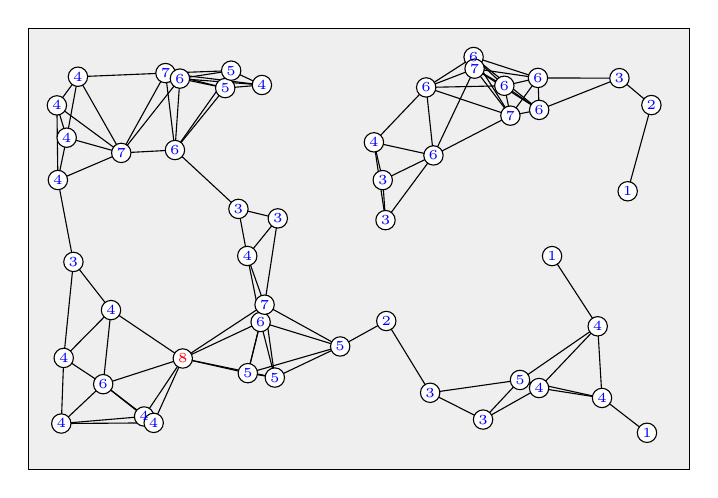
\begin{tikzpicture}[scale=1.4]
\fill[lightgray!25,draw=black] (0,0) rectangle (6,4);
\clip (0,0) rectangle (6,4);-
\draw [](0.26,3.3) -- (0.269,2.623);
\draw [](0.26,3.3) -- (0.349,3.007);
\draw [](0.26,3.3) -- (0.451,3.56);
\draw [](0.26,3.3) -- (0.844,2.869);
\draw [](0.269,2.623) -- (0.349,3.007);
\draw [](0.269,2.623) -- (0.41,1.88);
\draw [](0.269,2.623) -- (0.844,2.869);
\draw [](0.3,0.414) -- (0.322,1.009);
\draw [](0.3,0.414) -- (0.68,0.771);
\draw [](0.3,0.414) -- (1.051,0.478);
\draw [](0.3,0.414) -- (1.138,0.42);
\draw [](0.322,1.009) -- (0.41,1.88);
\draw [](0.322,1.009) -- (0.68,0.771);
\draw [](0.322,1.009) -- (0.751,1.443);
\draw [](0.349,3.007) -- (0.451,3.56);
\draw [](0.349,3.007) -- (0.844,2.869);
\draw [](0.41,1.88) -- (0.751,1.443);
\draw [](0.451,3.56) -- (0.844,2.869);
\draw [](0.451,3.56) -- (1.245,3.593);
\draw [](0.68,0.771) -- (0.751,1.443);
\draw [](0.68,0.771) -- (1.051,0.478);
\draw [](0.68,0.771) -- (1.138,0.42);
\draw [](0.68,0.771) -- (1.402,1.004);
\draw [](0.751,1.443) -- (1.402,1.004);
\draw [](0.844,2.869) -- (1.245,3.593);
\draw [](0.844,2.869) -- (1.331,2.895);
\draw [](0.844,2.869) -- (1.376,3.543);
\draw [](1.051,0.478) -- (1.138,0.42);
\draw [](1.051,0.478) -- (1.402,1.004);
\draw [](1.138,0.42) -- (1.402,1.004);
\draw [](1.245,3.593) -- (1.331,2.895);
\draw [](1.245,3.593) -- (1.376,3.543);
\draw [](1.245,3.593) -- (1.787,3.457);
\draw [](1.245,3.593) -- (1.841,3.615);
\draw [](1.245,3.593) -- (2.12,3.485);
\draw [](1.331,2.895) -- (1.376,3.543);
\draw [](1.331,2.895) -- (1.787,3.457);
\draw [](1.331,2.895) -- (1.841,3.615);
\draw [](1.331,2.895) -- (1.907,2.361);
\draw [](1.376,3.543) -- (1.787,3.457);
\draw [](1.376,3.543) -- (1.841,3.615);
\draw [](1.376,3.543) -- (2.12,3.485);
\draw [](1.402,1.004) -- (1.992,0.871);
\draw [](1.402,1.004) -- (2.108,1.335);
\draw [](1.402,1.004) -- (2.144,1.492);
\draw [](1.402,1.004) -- (2.237,0.831);
\draw [](1.787,3.457) -- (1.841,3.615);
\draw [](1.787,3.457) -- (2.12,3.485);
\draw [](1.841,3.615) -- (2.12,3.485);
\draw [](1.907,2.361) -- (1.987,1.934);
\draw [](1.907,2.361) -- (2.264,2.275);
\draw [](1.987,1.934) -- (2.108,1.335);
\draw [](1.987,1.934) -- (2.144,1.492);
\draw [](1.987,1.934) -- (2.264,2.275);
\draw [](1.992,0.871) -- (2.108,1.335);
\draw [](1.992,0.871) -- (2.144,1.492);
\draw [](1.992,0.871) -- (2.237,0.831);
\draw [](1.992,0.871) -- (2.83,1.113);
\draw [](2.108,1.335) -- (2.144,1.492);
\draw [](2.108,1.335) -- (2.237,0.831);
\draw [](2.108,1.335) -- (2.83,1.113);
\draw [](2.144,1.492) -- (2.237,0.831);
\draw [](2.144,1.492) -- (2.264,2.275);
\draw [](2.144,1.492) -- (2.83,1.113);
\draw [](2.237,0.831) -- (2.83,1.113);
\draw [](2.83,1.113) -- (3.248,1.344);
\draw [](3.136,2.965) -- (3.216,2.622);
\draw [](3.136,2.965) -- (3.241,2.259);
\draw [](3.136,2.965) -- (3.61,3.463);
\draw [](3.136,2.965) -- (3.676,2.846);
\draw [](3.216,2.622) -- (3.241,2.259);
\draw [](3.216,2.622) -- (3.676,2.846);
\draw [](3.241,2.259) -- (3.676,2.846);
\draw [](3.248,1.344) -- (3.646,0.693);
\draw [](3.61,3.463) -- (3.676,2.846);
\draw [](3.61,3.463) -- (4.04,3.739);
\draw [](3.61,3.463) -- (4.049,3.633);
\draw [](3.61,3.463) -- (4.319,3.478);
\draw [](3.61,3.463) -- (4.374,3.207);
\draw [](3.646,0.693) -- (4.126,0.45);
\draw [](3.646,0.693) -- (4.461,0.809);
\draw [](3.676,2.846) -- (4.049,3.633);
\draw [](3.676,2.846) -- (4.374,3.207);
\draw [](4.04,3.739) -- (4.049,3.633);
\draw [](4.04,3.739) -- (4.319,3.478);
\draw [](4.04,3.739) -- (4.374,3.207);
\draw [](4.04,3.739) -- (4.624,3.549);
\draw [](4.04,3.739) -- (4.635,3.259);
\draw [](4.049,3.633) -- (4.319,3.478);
\draw [](4.049,3.633) -- (4.374,3.207);
\draw [](4.049,3.633) -- (4.624,3.549);
\draw [](4.049,3.633) -- (4.635,3.259);
\draw [](4.126,0.45) -- (4.461,0.809);
\draw [](4.126,0.45) -- (4.634,0.736);
\draw [](4.319,3.478) -- (4.374,3.207);
\draw [](4.319,3.478) -- (4.624,3.549);
\draw [](4.319,3.478) -- (4.635,3.259);
\draw [](4.374,3.207) -- (4.624,3.549);
\draw [](4.374,3.207) -- (4.635,3.259);
\draw [](4.461,0.809) -- (4.634,0.736);
\draw [](4.461,0.809) -- (5.166,1.296);
\draw [](4.461,0.809) -- (5.205,0.646);
\draw [](4.624,3.549) -- (4.635,3.259);
\draw [](4.624,3.549) -- (5.363,3.547);
\draw [](4.634,0.736) -- (5.166,1.296);
\draw [](4.634,0.736) -- (5.205,0.646);
\draw [](4.635,3.259) -- (5.363,3.547);
\draw [](4.752,1.933) -- (5.166,1.296);
\draw [](5.166,1.296) -- (5.205,0.646);
\draw [](5.205,0.646) -- (5.613,0.33);
\draw [](5.363,3.547) -- (5.653,3.303);
\draw [](5.438,2.521) -- (5.653,3.303);
\fill [white,draw=black] (0.26,3.3) circle (2.5pt);
\fill [white,draw=black] (0.269,2.623) circle (2.5pt);
\fill [white,draw=black] (0.3,0.414) circle (2.5pt);
\fill [white,draw=black] (0.322,1.009) circle (2.5pt);
\fill [white,draw=black] (0.349,3.007) circle (2.5pt);
\fill [white,draw=black] (0.41,1.88) circle (2.5pt);
\fill [white,draw=black] (0.451,3.56) circle (2.5pt);
\fill [white,draw=black] (0.68,0.771) circle (2.5pt);
\fill [white,draw=black] (0.751,1.443) circle (2.5pt);
\fill [white,draw=black] (0.844,2.869) circle (2.5pt);
\fill [white,draw=black] (1.051,0.478) circle (2.5pt);
\fill [white,draw=black] (1.138,0.42) circle (2.5pt);
\fill [white,draw=black] (1.245,3.593) circle (2.5pt);
\fill [white,draw=black] (1.331,2.895) circle (2.5pt);
\fill [white,draw=black] (1.376,3.543) circle (2.5pt);
\fill [white,draw=black] (1.402,1.004) circle (2.5pt);
\fill [white,draw=black] (1.787,3.457) circle (2.5pt);
\fill [white,draw=black] (1.841,3.615) circle (2.5pt);
\fill [white,draw=black] (1.907,2.361) circle (2.5pt);
\fill [white,draw=black] (1.987,1.934) circle (2.5pt);
\fill [white,draw=black] (1.992,0.871) circle (2.5pt);
\fill [white,draw=black] (2.108,1.335) circle (2.5pt);
\fill [white,draw=black] (2.12,3.485) circle (2.5pt);
\fill [white,draw=black] (2.144,1.492) circle (2.5pt);
\fill [white,draw=black] (2.237,0.831) circle (2.5pt);
\fill [white,draw=black] (2.264,2.275) circle (2.5pt);
\fill [white,draw=black] (2.83,1.113) circle (2.5pt);
\fill [white,draw=black] (3.136,2.965) circle (2.5pt);
\fill [white,draw=black] (3.216,2.622) circle (2.5pt);
\fill [white,draw=black] (3.241,2.259) circle (2.5pt);
\fill [white,draw=black] (3.248,1.344) circle (2.5pt);
\fill [white,draw=black] (3.61,3.463) circle (2.5pt);
\fill [white,draw=black] (3.646,0.693) circle (2.5pt);
\fill [white,draw=black] (3.676,2.846) circle (2.5pt);
\fill [white,draw=black] (4.04,3.739) circle (2.5pt);
\fill [white,draw=black] (4.049,3.633) circle (2.5pt);
\fill [white,draw=black] (4.126,0.45) circle (2.5pt);
\fill [white,draw=black] (4.319,3.478) circle (2.5pt);
\fill [white,draw=black] (4.374,3.207) circle (2.5pt);
\fill [white,draw=black] (4.461,0.809) circle (2.5pt);
\fill [white,draw=black] (4.624,3.549) circle (2.5pt);
\fill [white,draw=black] (4.634,0.736) circle (2.5pt);
\fill [white,draw=black] (4.635,3.259) circle (2.5pt);
\fill [white,draw=black] (4.752,1.933) circle (2.5pt);
\fill [white,draw=black] (5.166,1.296) circle (2.5pt);
\fill [white,draw=black] (5.205,0.646) circle (2.5pt);
\fill [white,draw=black] (5.363,3.547) circle (2.5pt);
\fill [white,draw=black] (5.438,2.521) circle (2.5pt);
\fill [white,draw=black] (5.613,0.33) circle (2.5pt);
\fill [white,draw=black] (5.653,3.303) circle (2.5pt);
\node [blue] at (0.26,3.3) {\tiny $4$};
\node [blue] at (0.269,2.623) {\tiny $4$};
\node [blue] at (0.3,0.414) {\tiny $4$};
\node [blue] at (0.322,1.009) {\tiny $4$};
\node [blue] at (0.349,3.007) {\tiny $4$};
\node [blue] at (0.41,1.88) {\tiny $3$};
\node [blue] at (0.451,3.56) {\tiny $4$};
\node [blue] at (0.68,0.771) {\tiny $6$};
\node [blue] at (0.751,1.443) {\tiny $4$};
\node [blue] at (0.844,2.869) {\tiny $7$};
\node [blue] at (1.051,0.478) {\tiny $4$};
\node [blue] at (1.138,0.42) {\tiny $4$};
\node [blue] at (1.245,3.593) {\tiny $7$};
\node [blue] at (1.331,2.895) {\tiny $6$};
\node [blue] at (1.376,3.543) {\tiny $6$};
\node [red] at (1.402,1.004) {\tiny $8$};
\node [blue] at (1.787,3.457) {\tiny $5$};
\node [blue] at (1.841,3.615) {\tiny $5$};
\node [blue] at (1.907,2.361) {\tiny $3$};
\node [blue] at (1.987,1.934) {\tiny $4$};
\node [blue] at (1.992,0.871) {\tiny $5$};
\node [blue] at (2.108,1.335) {\tiny $6$};
\node [blue] at (2.12,3.485) {\tiny $4$};
\node [blue] at (2.144,1.492) {\tiny $7$};
\node [blue] at (2.237,0.831) {\tiny $5$};
\node [blue] at (2.264,2.275) {\tiny $3$};
\node [blue] at (2.83,1.113) {\tiny $5$};
\node [blue] at (3.136,2.965) {\tiny $4$};
\node [blue] at (3.216,2.622) {\tiny $3$};
\node [blue] at (3.241,2.259) {\tiny $3$};
\node [blue] at (3.248,1.344) {\tiny $2$};
\node [blue] at (3.61,3.463) {\tiny $6$};
\node [blue] at (3.646,0.693) {\tiny $3$};
\node [blue] at (3.676,2.846) {\tiny $6$};
\node [blue] at (4.04,3.739) {\tiny $6$};
\node [blue] at (4.049,3.633) {\tiny $7$};
\node [blue] at (4.126,0.45) {\tiny $3$};
\node [blue] at (4.319,3.478) {\tiny $6$};
\node [blue] at (4.374,3.207) {\tiny $7$};
\node [blue] at (4.461,0.809) {\tiny $5$};
\node [blue] at (4.624,3.549) {\tiny $6$};
\node [blue] at (4.634,0.736) {\tiny $4$};
\node [blue] at (4.635,3.259) {\tiny $6$};
\node [blue] at (4.752,1.933) {\tiny $1$};
\node [blue] at (5.166,1.296) {\tiny $4$};
\node [blue] at (5.205,0.646) {\tiny $4$};
\node [blue] at (5.363,3.547) {\tiny $3$};
\node [blue] at (5.438,2.521) {\tiny $1$};
\node [blue] at (5.613,0.33) {\tiny $1$};
\node [blue] at (5.653,3.303) {\tiny $2$};
\end{tikzpicture}

\end{center}
\caption{Illustration of the Resulting Graph. The numbers on the points represent the number of neighbours. The number in red represents the point with the largest number of neighbours.}
\label{fig:aa1}
\end{figure}


This graph is represented via adjacency lists. The adjacency lists have an advantage over an adjacency matrix as linked lists can be used to considerably reduce the memory footprint in sparse graphs. It also allows for faster sequential access to the neighbours of any given point. These linked lists share similarities to the half-edge structure, in which each node represents a unidirectional edge that contains a pointer to its counterpart.

It is noteworthy that the graph can reach $\bigo(n^2)$ edges if the points are all very close together and/or the minimum distance is large enough. This case coupled with the fact that the adjacency linked lists occupy more space per edge than an adjacency matrix, the space needed to keep the graph in memory can be potentially too high for some machines to handle larger instances of the problem. 

\subsection{Set Cover}
The second step to the algorithm is to chose a small subset of vertices whose neighbours unions are equal to the whole set of vertices of the graph. This is known as \emph{set cover}, and its solution can be approximated using a greedy approach \cite{approxalgos}. Starting with the whole uncovered graph, the point with the largest number of uncovered neighbours is selected. This is done iteratively until no uncovered points remain on the graph. This approach approximates the number of points to within $m \ln{n}$ points, were $m$ is the optimal number.

At each step of this algorithm, one point $p$ and all its neighbours and respective edges must be removed from the graph. This is done by iterating through the adjacency lists of the neighbours of $p$ and deleting all the connections to their neighbours (second-degree neighbours of $p$). This operation takes exactly $\bigo(n)$ time where $n$ is proportional to the number of edges to be deleted. Figure \ref{fig:aa2} illustrates the graph after the first iteration:

\begin{figure}[H]
\begin{center}
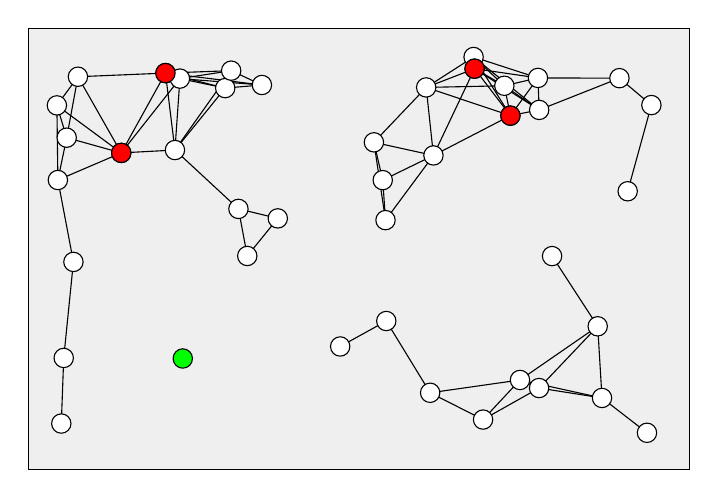
\begin{tikzpicture}[scale=1.4]
\fill[lightgray!25,draw=black] (0,0) rectangle (6,4);
\clip (0,0) rectangle (6,4);
\draw [](0.26,3.3) -- (0.269,2.623);
\draw [](0.26,3.3) -- (0.349,3.007);
\draw [](0.26,3.3) -- (0.451,3.56);
\draw [](0.26,3.3) -- (0.844,2.869);
\draw [](0.269,2.623) -- (0.349,3.007);
\draw [](0.269,2.623) -- (0.41,1.88);
\draw [](0.269,2.623) -- (0.844,2.869);
\draw [](0.3,0.414) -- (0.322,1.009);
\draw [](0.322,1.009) -- (0.41,1.88);
\draw [](0.349,3.007) -- (0.451,3.56);
\draw [](0.349,3.007) -- (0.844,2.869);
\draw [](0.451,3.56) -- (0.844,2.869);
\draw [](0.451,3.56) -- (1.245,3.593);
\draw [](0.844,2.869) -- (1.245,3.593);
\draw [](0.844,2.869) -- (1.331,2.895);
\draw [](0.844,2.869) -- (1.376,3.543);
\draw [](1.245,3.593) -- (1.331,2.895);
\draw [](1.245,3.593) -- (1.376,3.543);
\draw [](1.245,3.593) -- (1.787,3.457);
\draw [](1.245,3.593) -- (1.841,3.615);
\draw [](1.245,3.593) -- (2.12,3.485);
\draw [](1.331,2.895) -- (1.376,3.543);
\draw [](1.331,2.895) -- (1.787,3.457);
\draw [](1.331,2.895) -- (1.841,3.615);
\draw [](1.331,2.895) -- (1.907,2.361);
\draw [](1.376,3.543) -- (1.787,3.457);
\draw [](1.376,3.543) -- (1.841,3.615);
\draw [](1.376,3.543) -- (2.12,3.485);
\draw [](1.787,3.457) -- (1.841,3.615);
\draw [](1.787,3.457) -- (2.12,3.485);
\draw [](1.841,3.615) -- (2.12,3.485);
\draw [](1.907,2.361) -- (1.987,1.934);
\draw [](1.907,2.361) -- (2.264,2.275);
\draw [](1.987,1.934) -- (2.264,2.275);
\draw [](2.83,1.113) -- (3.248,1.344);
\draw [](3.136,2.965) -- (3.216,2.622);
\draw [](3.136,2.965) -- (3.241,2.259);
\draw [](3.136,2.965) -- (3.61,3.463);
\draw [](3.136,2.965) -- (3.676,2.846);
\draw [](3.216,2.622) -- (3.241,2.259);
\draw [](3.216,2.622) -- (3.676,2.846);
\draw [](3.241,2.259) -- (3.676,2.846);
\draw [](3.248,1.344) -- (3.646,0.693);
\draw [](3.61,3.463) -- (3.676,2.846);
\draw [](3.61,3.463) -- (4.04,3.739);
\draw [](3.61,3.463) -- (4.049,3.633);
\draw [](3.61,3.463) -- (4.319,3.478);
\draw [](3.61,3.463) -- (4.374,3.207);
\draw [](3.646,0.693) -- (4.126,0.45);
\draw [](3.646,0.693) -- (4.461,0.809);
\draw [](3.676,2.846) -- (4.049,3.633);
\draw [](3.676,2.846) -- (4.374,3.207);
\draw [](4.04,3.739) -- (4.049,3.633);
\draw [](4.04,3.739) -- (4.319,3.478);
\draw [](4.04,3.739) -- (4.374,3.207);
\draw [](4.04,3.739) -- (4.624,3.549);
\draw [](4.04,3.739) -- (4.635,3.259);
\draw [](4.049,3.633) -- (4.319,3.478);
\draw [](4.049,3.633) -- (4.374,3.207);
\draw [](4.049,3.633) -- (4.624,3.549);
\draw [](4.049,3.633) -- (4.635,3.259);
\draw [](4.126,0.45) -- (4.461,0.809);
\draw [](4.126,0.45) -- (4.634,0.736);
\draw [](4.319,3.478) -- (4.374,3.207);
\draw [](4.319,3.478) -- (4.624,3.549);
\draw [](4.319,3.478) -- (4.635,3.259);
\draw [](4.374,3.207) -- (4.624,3.549);
\draw [](4.374,3.207) -- (4.635,3.259);
\draw [](4.461,0.809) -- (4.634,0.736);
\draw [](4.461,0.809) -- (5.166,1.296);
\draw [](4.461,0.809) -- (5.205,0.646);
\draw [](4.624,3.549) -- (4.635,3.259);
\draw [](4.624,3.549) -- (5.363,3.547);
\draw [](4.634,0.736) -- (5.166,1.296);
\draw [](4.634,0.736) -- (5.205,0.646);
\draw [](4.635,3.259) -- (5.363,3.547);
\draw [](4.752,1.933) -- (5.166,1.296);
\draw [](5.166,1.296) -- (5.205,0.646);
\draw [](5.205,0.646) -- (5.613,0.33);
\draw [](5.363,3.547) -- (5.653,3.303);
\draw [](5.438,2.521) -- (5.653,3.303);
\fill [white,draw=black] (0.26,3.3) circle (2.5pt);
\fill [white,draw=black] (0.269,2.623) circle (2.5pt);
\fill [white,draw=black] (0.3,0.414) circle (2.5pt);
\fill [white,draw=black] (0.322,1.009) circle (2.5pt);
\fill [white,draw=black] (0.349,3.007) circle (2.5pt);
\fill [white,draw=black] (0.41,1.88) circle (2.5pt);
\fill [white,draw=black] (0.451,3.56) circle (2.5pt);
\fill [white,draw=black] (0.844,2.869) circle (2.5pt);
\fill [white,draw=black] (1.245,3.593) circle (2.5pt);
\fill [white,draw=black] (1.331,2.895) circle (2.5pt);
\fill [white,draw=black] (1.376,3.543) circle (2.5pt);
\fill [white,draw=black] (1.787,3.457) circle (2.5pt);
\fill [white,draw=black] (1.841,3.615) circle (2.5pt);
\fill [white,draw=black] (1.907,2.361) circle (2.5pt);
\fill [white,draw=black] (1.987,1.934) circle (2.5pt);
\fill [white,draw=black] (2.12,3.485) circle (2.5pt);
\fill [white,draw=black] (2.264,2.275) circle (2.5pt);
\fill [white,draw=black] (2.83,1.113) circle (2.5pt);
\fill [white,draw=black] (3.136,2.965) circle (2.5pt);
\fill [white,draw=black] (3.216,2.622) circle (2.5pt);
\fill [white,draw=black] (3.241,2.259) circle (2.5pt);
\fill [white,draw=black] (3.248,1.344) circle (2.5pt);
\fill [white,draw=black] (3.61,3.463) circle (2.5pt);
\fill [white,draw=black] (3.646,0.693) circle (2.5pt);
\fill [white,draw=black] (3.676,2.846) circle (2.5pt);
\fill [white,draw=black] (4.04,3.739) circle (2.5pt);
\fill [white,draw=black] (4.049,3.633) circle (2.5pt);
\fill [white,draw=black] (4.126,0.45) circle (2.5pt);
\fill [white,draw=black] (4.319,3.478) circle (2.5pt);
\fill [white,draw=black] (4.374,3.207) circle (2.5pt);
\fill [white,draw=black] (4.461,0.809) circle (2.5pt);
\fill [white,draw=black] (4.624,3.549) circle (2.5pt);
\fill [white,draw=black] (4.634,0.736) circle (2.5pt);
\fill [white,draw=black] (4.635,3.259) circle (2.5pt);
\fill [white,draw=black] (4.752,1.933) circle (2.5pt);
\fill [white,draw=black] (5.166,1.296) circle (2.5pt);
\fill [white,draw=black] (5.205,0.646) circle (2.5pt);
\fill [white,draw=black] (5.363,3.547) circle (2.5pt);
\fill [white,draw=black] (5.438,2.521) circle (2.5pt);
\fill [white,draw=black] (5.613,0.33) circle (2.5pt);
\fill [white,draw=black] (5.653,3.303) circle (2.5pt);
%\node [blue] at (0.26,3.3) {\tiny $4$};
%\node [blue] at (0.269,2.623) {\tiny $4$};
%\node [blue] at (0.3,0.414) {\tiny $1$};
%\node [blue] at (0.322,1.009) {\tiny $2$};
%\node [blue] at (0.349,3.007) {\tiny $4$};
%\node [blue] at (0.41,1.88) {\tiny $2$};
%\node [blue] at (0.451,3.56) {\tiny $4$};
%\node [red] at (0.844,2.869) {\tiny $7$};
%\node [red] at (1.245,3.593) {\tiny $7$};
%\node [blue] at (1.331,2.895) {\tiny $6$};
%\node [blue] at (1.376,3.543) {\tiny $6$};
%\node [blue] at (1.787,3.457) {\tiny $5$};
%\node [blue] at (1.841,3.615) {\tiny $5$};
%\node [blue] at (1.907,2.361) {\tiny $3$};
%\node [blue] at (1.987,1.934) {\tiny $2$};
%\node [blue] at (2.12,3.485) {\tiny $4$};
%\node [blue] at (2.264,2.275) {\tiny $2$};
%\node [blue] at (2.83,1.113) {\tiny $1$};
%\node [blue] at (3.136,2.965) {\tiny $4$};
%\node [blue] at (3.216,2.622) {\tiny $3$};
%\node [blue] at (3.241,2.259) {\tiny $3$};
%\node [blue] at (3.248,1.344) {\tiny $2$};
%\node [blue] at (3.61,3.463) {\tiny $6$};
%\node [blue] at (3.646,0.693) {\tiny $3$};
%\node [blue] at (3.676,2.846) {\tiny $6$};
%\node [blue] at (4.04,3.739) {\tiny $6$};
%\node [red] at (4.049,3.633) {\tiny $7$};
%\node [blue] at (4.126,0.45) {\tiny $3$};
%\node [blue] at (4.319,3.478) {\tiny $6$};
%\node [red] at (4.374,3.207) {\tiny $7$};
%\node [blue] at (4.461,0.809) {\tiny $5$};
%\node [blue] at (4.624,3.549) {\tiny $6$};
%\node [blue] at (4.634,0.736) {\tiny $4$};
%\node [blue] at (4.635,3.259) {\tiny $6$};
%\node [blue] at (4.752,1.933) {\tiny $1$};
%\node [blue] at (5.166,1.296) {\tiny $4$};
%\node [blue] at (5.205,0.646) {\tiny $4$};
%\node [blue] at (5.363,3.547) {\tiny $3$};
%\node [blue] at (5.438,2.521) {\tiny $1$};
%\node [blue] at (5.613,0.33) {\tiny $1$};
%\node [blue] at (5.653,3.303) {\tiny $2$};
\fill [red,draw=black] (0.844,2.869) circle (2.5pt);
%\node [red] at (0.844,2.869) {\tiny $7$};
\fill [red,draw=black] (1.245,3.593) circle (2.5pt);
%\node [red] at (1.245,3.593) {\tiny $7$};
\fill [red,draw=black] (4.049,3.633) circle (2.5pt);
%\node [red] at (4.049,3.633) {\tiny $7$};
\fill [red,draw=black] (4.374,3.207) circle (2.5pt);
%\node [red] at (4.374,3.207) {\tiny $7$};
\fill [green,draw=black] (1.402,1.004) circle (2.5pt);
\end{tikzpicture}

\end{center}
\caption{Illustration of the state of the graph after the first iteration. Any of the red points is to be removed in the next iteration, as they have the largest amount of neighbours.}
\label{fig:aa2}
\end{figure}


After all the points are covered, the collection of selected centres makes the subset of centroids that is displayed as the final output. The cardinality of this set does not exceed the approximation as described above.

\begin{figure}[H]
\begin{center}
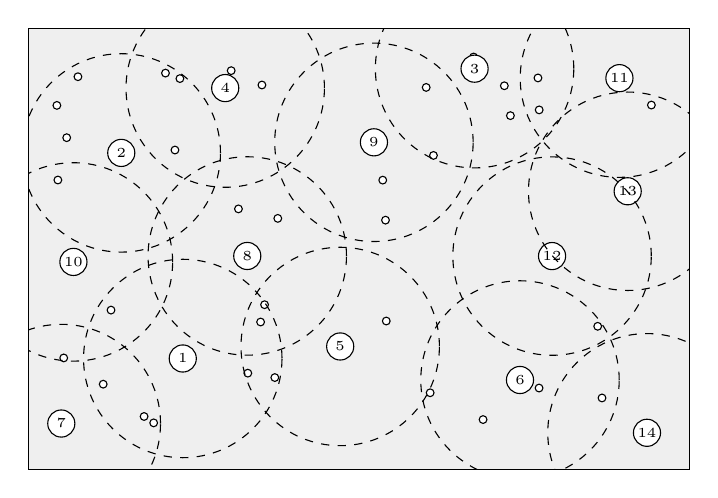
\begin{tikzpicture}[scale=1.4]
\fill[lightgray!25,draw=black] (0,0) rectangle (6,4);
\clip (0,0) rectangle (6,4);


\fill [white,draw=black] (0.26,3.3) circle (1pt);
\fill [white,draw=black] (0.269,2.623) circle (1pt);
\fill [white,draw=black] (0.3,0.414) circle (1pt);
\fill [white,draw=black] (0.322,1.009) circle (1pt);
\fill [white,draw=black] (0.349,3.007) circle (1pt);
\fill [white,draw=black] (0.41,1.88) circle (1pt);
\fill [white,draw=black] (0.451,3.56) circle (1pt);
\fill [white,draw=black] (0.68,0.771) circle (1pt);
\fill [white,draw=black] (0.751,1.443) circle (1pt);
\fill [white,draw=black] (0.844,2.869) circle (1pt);
\fill [white,draw=black] (1.051,0.478) circle (1pt);
\fill [white,draw=black] (1.138,0.42) circle (1pt);
\fill [white,draw=black] (1.245,3.593) circle (1pt);
\fill [white,draw=black] (1.331,2.895) circle (1pt);
\fill [white,draw=black] (1.376,3.543) circle (1pt);
\fill [white,draw=black] (1.402,1.004) circle (1pt);
\fill [white,draw=black] (1.787,3.457) circle (1pt);
\fill [white,draw=black] (1.841,3.615) circle (1pt);
\fill [white,draw=black] (1.907,2.361) circle (1pt);
\fill [white,draw=black] (1.987,1.934) circle (1pt);
\fill [white,draw=black] (1.992,0.871) circle (1pt);
\fill [white,draw=black] (2.108,1.335) circle (1pt);
\fill [white,draw=black] (2.12,3.485) circle (1pt);
\fill [white,draw=black] (2.144,1.492) circle (1pt);
\fill [white,draw=black] (2.237,0.831) circle (1pt);
\fill [white,draw=black] (2.264,2.275) circle (1pt);
\fill [white,draw=black] (2.83,1.113) circle (1pt);
\fill [white,draw=black] (3.136,2.965) circle (1pt);
\fill [white,draw=black] (3.216,2.622) circle (1pt);
\fill [white,draw=black] (3.241,2.259) circle (1pt);
\fill [white,draw=black] (3.248,1.344) circle (1pt);
\fill [white,draw=black] (3.61,3.463) circle (1pt);
\fill [white,draw=black] (3.646,0.693) circle (1pt);
\fill [white,draw=black] (3.676,2.846) circle (1pt);
\fill [white,draw=black] (4.04,3.739) circle (1pt);
\fill [white,draw=black] (4.049,3.633) circle (1pt);
\fill [white,draw=black] (4.126,0.45) circle (1pt);
\fill [white,draw=black] (4.319,3.478) circle (1pt);
\fill [white,draw=black] (4.374,3.207) circle (1pt);
\fill [white,draw=black] (4.461,0.809) circle (1pt);
\fill [white,draw=black] (4.624,3.549) circle (1pt);
\fill [white,draw=black] (4.634,0.736) circle (1pt);
\fill [white,draw=black] (4.635,3.259) circle (1pt);
\fill [white,draw=black] (4.752,1.933) circle (1pt);
\fill [white,draw=black] (5.166,1.296) circle (1pt);
\fill [white,draw=black] (5.205,0.646) circle (1pt);
\fill [white,draw=black] (5.363,3.547) circle (1pt);
\fill [white,draw=black] (5.438,2.521) circle (1pt);
\fill [white,draw=black] (5.613,0.33) circle (1pt);
\fill [white,draw=black] (5.653,3.303) circle (1pt);


\fill [white,draw=black] (1.402,1.004) circle (3.5pt);
\node [black] at (1.402,1.004) {\tiny $1$};
\fill [white,draw=black] (0.844,2.869) circle (3.5pt);
\node [black] at (0.844,2.869) {\tiny $2$};
\fill [white,draw=black] (4.049,3.633) circle (3.5pt);
\node [black] at (4.049,3.633) {\tiny $3$};
\fill [white,draw=black] (1.787,3.457) circle (3.5pt);
\node [black] at (1.787,3.457) {\tiny $4$};
\fill [white,draw=black] (2.83,1.113) circle (3.5pt);
\node [black] at (2.83,1.113) {\tiny $5$};
\fill [white,draw=black] (4.461,0.809) circle (3.5pt);
\node [black] at (4.461,0.809) {\tiny $6$};
\fill [white,draw=black] (0.3,0.414) circle (3.5pt);
\node [black] at (0.3,0.414) {\tiny $7$};
\fill [white,draw=black] (1.987,1.934) circle (3.5pt);
\node [black] at (1.987,1.934) {\tiny $8$};
\fill [white,draw=black] (3.136,2.965) circle (3.5pt);
\node [black] at (3.136,2.965) {\tiny $9$};
\fill [white,draw=black] (0.41,1.88) circle (3.5pt);
\node [black] at (0.41,1.88) {\tiny $10$};
\fill [white,draw=black] (5.363,3.547) circle (3.5pt);
\node [black] at (5.363,3.547) {\tiny $11$};
\fill [white,draw=black] (4.752,1.933) circle (3.5pt);
\node [black] at (4.752,1.933) {\tiny $12$};
\fill [white,draw=black] (5.438,2.521) circle (3.5pt);
\node [black] at (5.438,2.521) {\tiny $13$};
\fill [white,draw=black] (5.613,0.33) circle (3.5pt);
\node [black] at (5.613,0.33) {\tiny $14$};
\draw [dashed] (1.402,1.004) circle (0.9);
\draw [dashed] (0.844,2.869) circle (0.9);
\draw [dashed] (4.049,3.633) circle (0.9);
\draw [dashed] (1.787,3.457) circle (0.9);
\draw [dashed] (2.83,1.113) circle (0.9);
\draw [dashed] (4.461,0.809) circle (0.9);
\draw [dashed] (0.3,0.414) circle (0.9);
\draw [dashed] (1.987,1.934) circle (0.9);
\draw [dashed] (3.136,2.965) circle (0.9);
\draw [dashed] (0.41,1.88) circle (0.9);
\draw [dashed] (5.363,3.547) circle (0.9);
\draw [dashed] (4.752,1.933) circle (0.9);
\draw [dashed] (5.438,2.521) circle (0.9);
\draw [dashed] (5.613,0.33) circle (0.9);

\end{tikzpicture}

\end{center}
\caption{Illustration of the state of the final chosen set. The larger points are the chosen set, and the numbers represent the order in which they are chosen.}
\label{fig:aa3}


\end{figure}

\subsection{Results}
This section reports both approaches (\kdtrees and line sweeping) to the graph building portion of the algorithm. The implementations differ from each other only in the range search algorithm they use to build the proximity graph. This is done because the graph building stage has the highest time complexity, and is therefore expected to be the bottleneck. In fact, running a code profiler shows that the graph building stage takes 98\% of the CPU-time, with the time taken to run the set cover algorithm stage being negligible.

For the tests in this section, the given value of $d$ is the minimum distance between points, therefore radius of the covering disks. It is given as a percentage of the largest dimension of the window, as this value is easier to adjust and analyse by a human user.
Figure \ref{fig:sweden_dist} shows the outputs for different values of $d$ for a set of points of interest in Sweden. The data was obtained from the \href{http://www.math.uwaterloo.ca/tsp/world/swpoints.html}{University of Waterloo, Ontario, Canada}\cite{waterloo_sweden}.

\begin{figure}[!h] 
  \begin{subfigure}[b]{0.24\linewidth}
		\centering
		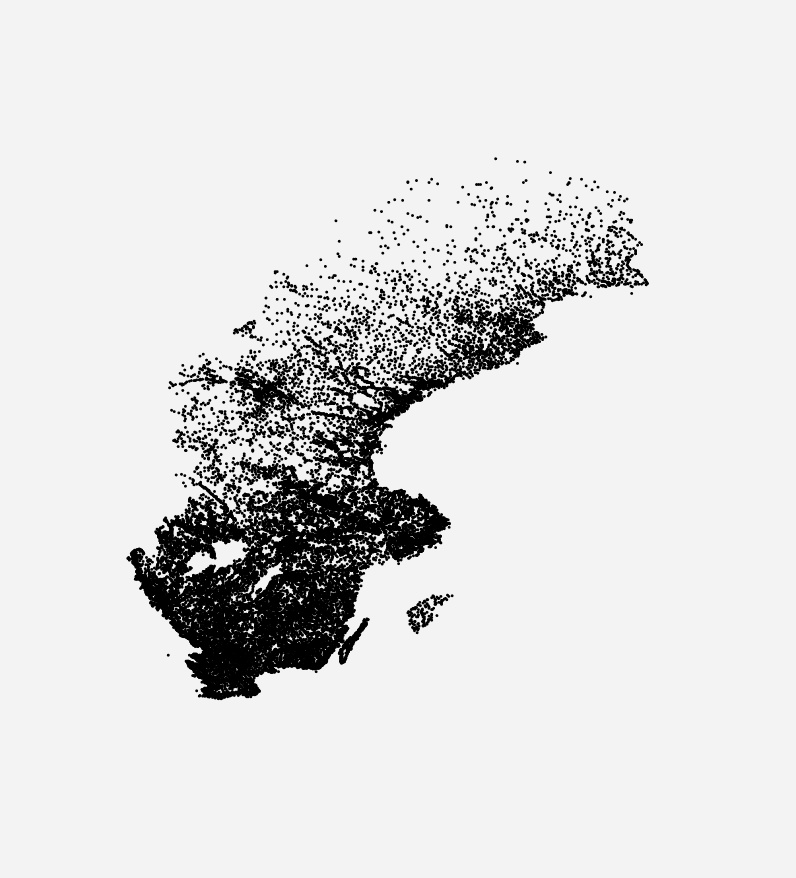
\includegraphics[width=0.9\linewidth]{Pictures/sweden} 
		\caption{\small Original Set} 
		\label{fig:or_sweden} 
		\vspace{4ex}
  \end{subfigure}
  \begin{subfigure}[b]{0.24\linewidth}
    \centering
    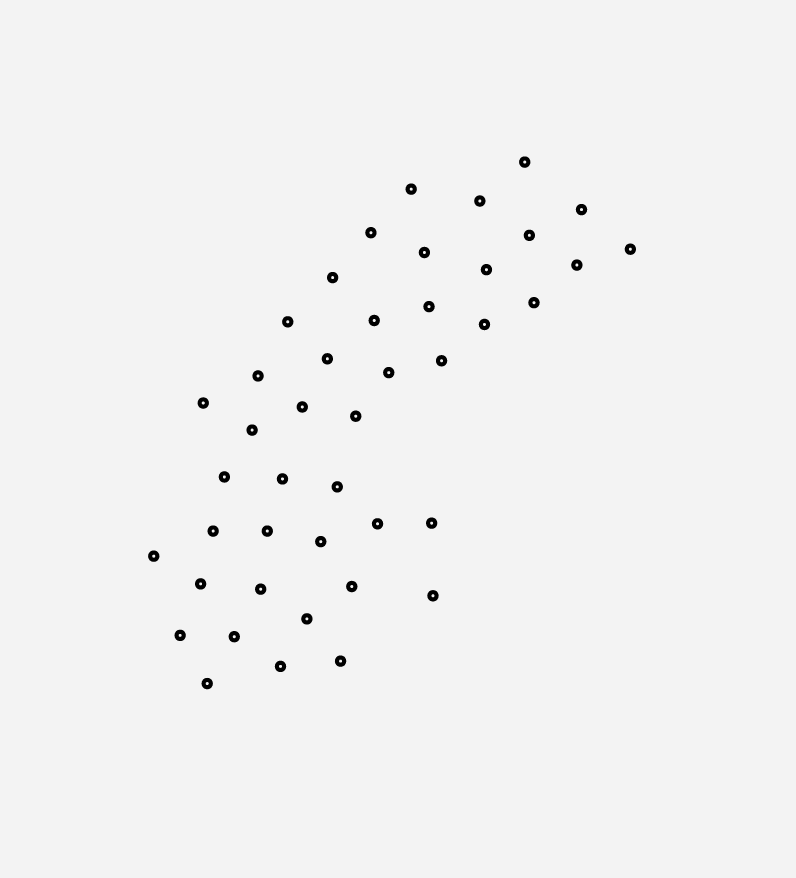
\includegraphics[width=0.9\linewidth]{Pictures/10_sweden} 
	\caption{\small $d=10\%$} 
    \label{fig:10_sweden} 
    \vspace{4ex}
  \end{subfigure}%% 
  \begin{subfigure}[b]{0.24\linewidth}
    \centering
    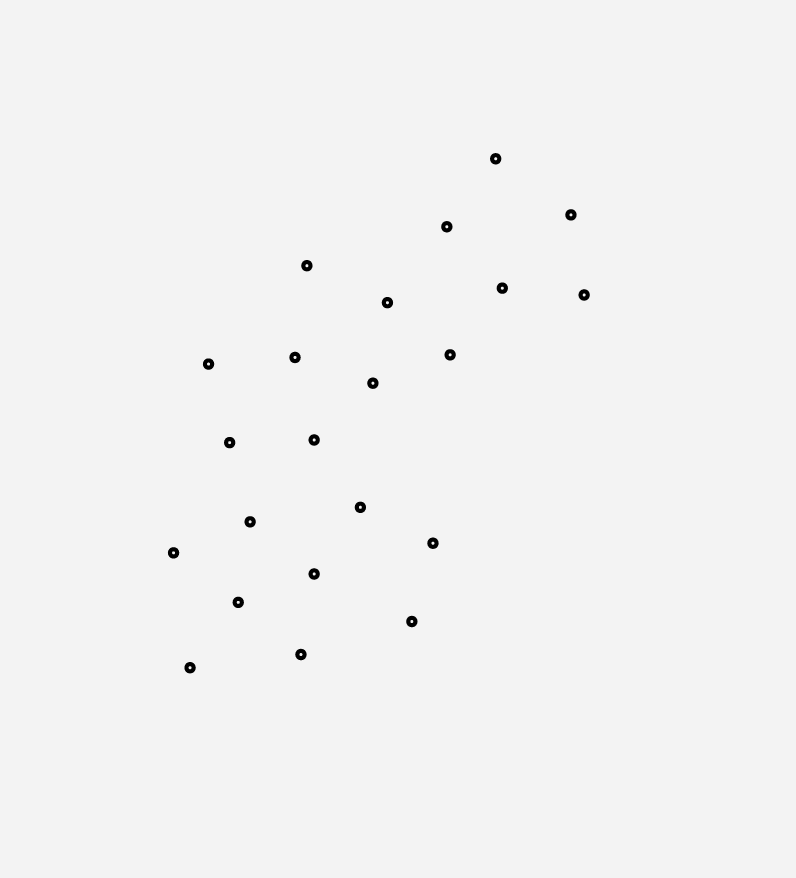
\includegraphics[width=0.9\linewidth]{Pictures/15_sweden} 
    \caption{\small $d=15\%$} 
    \label{fig:15_sweden} 
    \vspace{4ex}
  \end{subfigure}
  \begin{subfigure}[b]{0.24\linewidth}
  	\centering
  	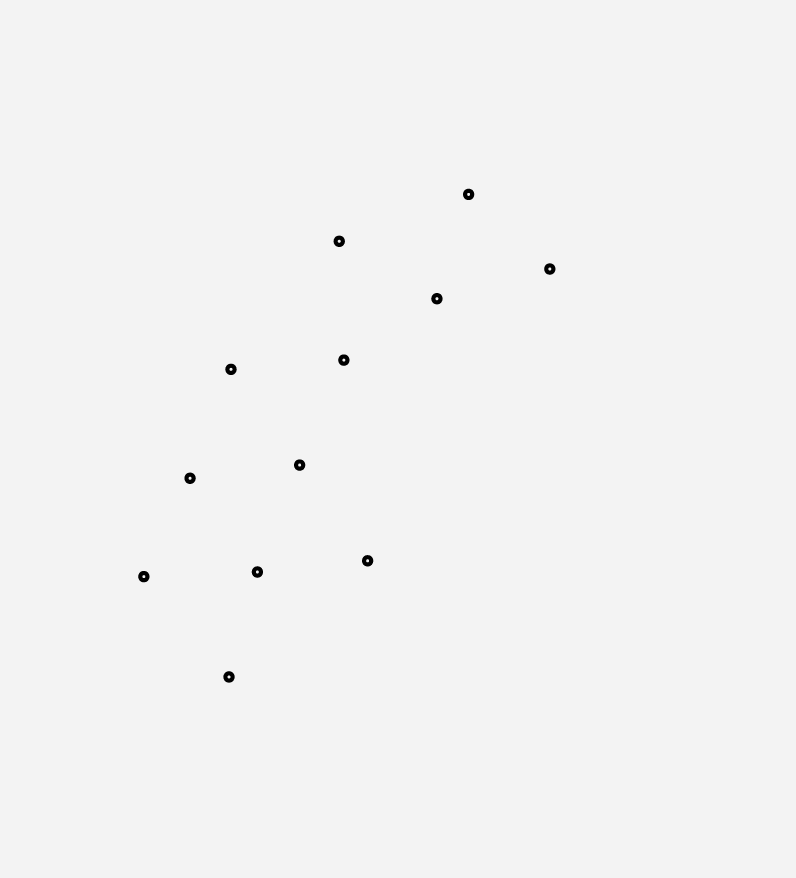
\includegraphics[width=0.9\linewidth]{Pictures/20_sweden} 
  	\caption{\small $d=20\%$} 
  	\label{fig:20_sweden} 
  	\vspace{4ex}
  \end{subfigure}
  \caption[Selected subsets from both graph building algorithms]{Selected subsets from both graph building algorithms.}
  \label{fig:sweden_dist} 
\end{figure}


By analysing images of a few real-world examples, the values for the minimum distance $d$ were agreed to be given as a value between 10\% and 15\% of the largest dimension of the window. These values give the subsets that were deemed as the easiest to look at without losing sense of shape of the area. The performance tests still use the value of 20\% to test the algorithms under less favourable conditions, since the larger the value of $d$, the denser and more time is required to build the proximity graph. 

Since this approach is more interesting for the web application from a coputational time point of view, a new set of benchmark tests were defined. Both uniform and clustered inputs are tested. The uniform inputs are a simple collection of $N$ points whose Cartesian coordinates are randomly chosen between $0$ and $100$. The clustered inputs are generated by choosing a random number of points $s$ between 10 to 20 points. Each of these points acts as a centre and is chosen by randomly generating two Cartesian coordinates between 0 and 100. Around each of these, $N/s$ points were generated by randomly choosing an angle $\Theta$ (between $0$ and $2\pi$) and a distance $\rho$ (between $10$ and $20$), which represent the polar coordinates around their respective central point. These tests generate circular clusters, with more density towards the centre. Each test is performed 30 times, with shared seeds between the algorithms. The times listed do include the input scanning. All algorithms are implemented using ANSI C89 and compiled using \emph{gcc 5.1.0}. The programs were ran on a machine with a Intel i7 Dual-Core, 2GHz processor, with a 8 GB, 1600 MHz memory and Arch Linux 3.14.4 x64 as its operating system.

The first test performed benchmarked both line sweep and \kdtree range search algorithms for the proximity graph construction. The results are shown in Figure \ref{fig:ls_kd_t}. As the Figure shows, the line sweep method performs faster in both the uniform and the clustered data. The lower expected complexity of the \kdtrees does not compensate the larger overhead in their construction. It can also be seen that both algorithms become slower the larger the number of points, as was expected.

Building a proximity graph with 30000 vertices has the potential to need $30000^2$ edges, making these algorithms very memory intensive. Even with adjacency lists instead of an adjacency matrix, the inputs can generate a instance where every point must be connected to every other point. In this case, the advantage of the adjacency lists for sparse graphs is lost, and the program exceeds the RAM limit given by the operating system. This occurs more frequently for larger values of $d$ and $N$, with the smallest case recorded being of $N=25000$ and $d=0.2$ on a clustered input that generated most clusters on top of each other, concentrating most points within a circle of a small radius, where most of them had over 20000 neighbours. However this case is somewhat rare, and only occurs under very specific circumstances and did not occur during the tests displayed. Figure \ref{fig:ls_kd_s} shows the amount of memory used by both algorithms on the tests performed. 
The lines for both algorithms overlap, since applying both methods to any given case gives the same proximity graph, as it is unique. 

However, the final set may not be the same. The coverage algorithm picks the points with most neighbours. Since two different points may have the same number of neighbours, and the two algorithms sort the points in two different ways, there may occur a case where the sets are completely different, based on which point is selected first in case of a draw. The values still fall bellow the upper bound for the approximation factor, and no algorithm should have the advantage over the other. Figure \ref{fig:ls_kd_k} shows the number of points selected by each algorithm in the same instances as above. The figure shows that the number of selected points $k$ does not seem to vary very much with $N$ for the same values of $d$. In fact, the growth of the value of $k$ seems to suggest an asymptotic approach to a fixed value. This happens because there is a limit to how many circles can be placed in an area without any of them containing the centres of the others. 

\begin{figure}[!h] 
	\centering
    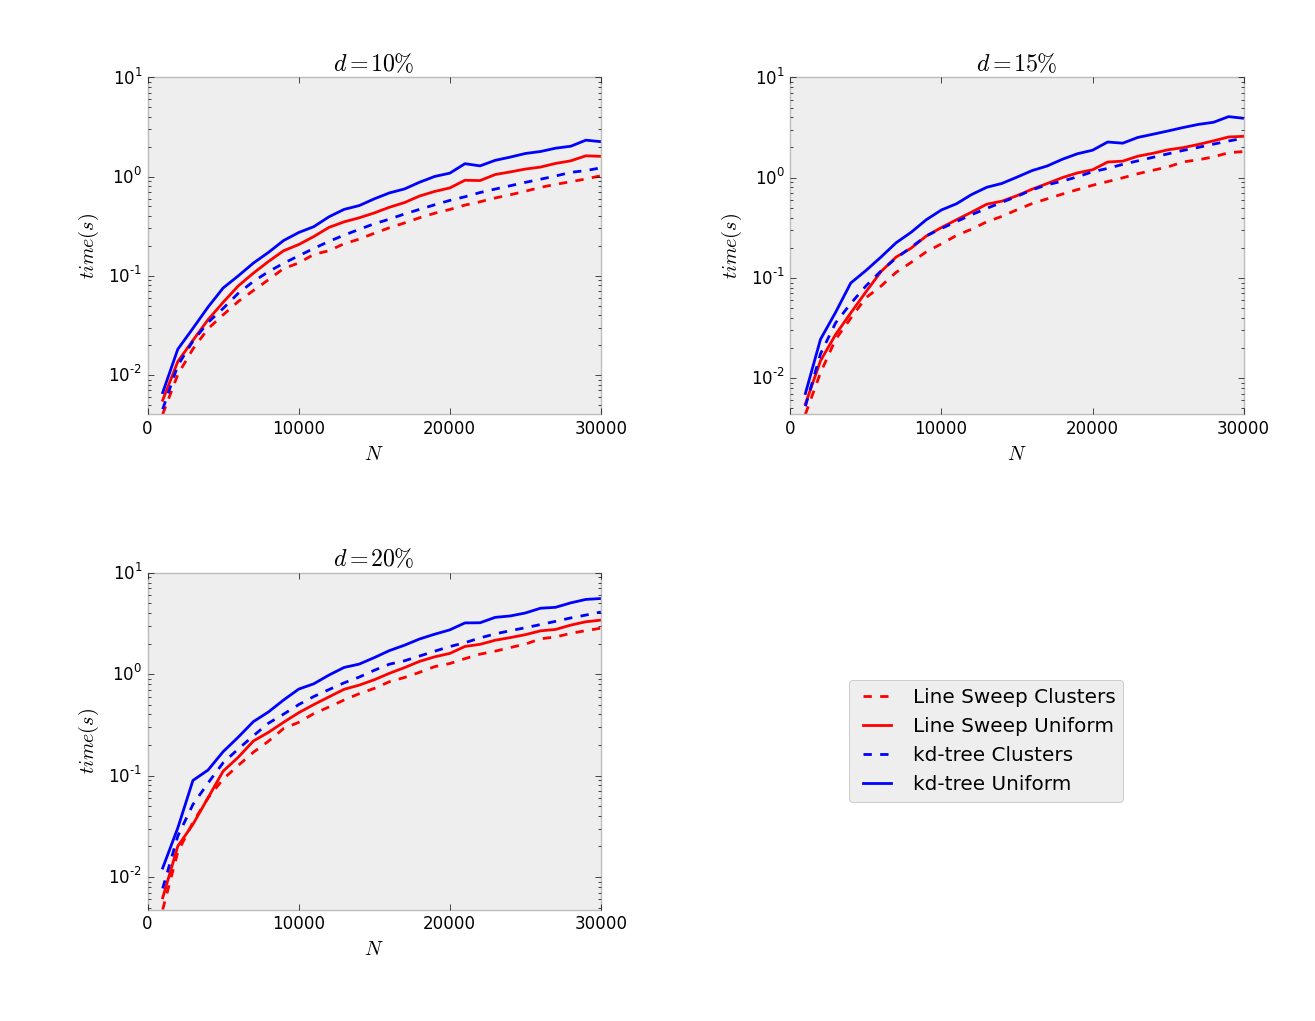
\includegraphics[width=\linewidth]{Pictures/ls_kd_t}
    \caption[CPU-time for Line Sweep and $k$-d Tree range search.]{CPU-time for both proximity graph algorithms on uniform and clustered inputs for different values of $d$.}
    \label{fig:ls_kd_t} 
\end{figure}


\begin{figure}[!h] 
	\centering 
	\vspace{-10pt}
    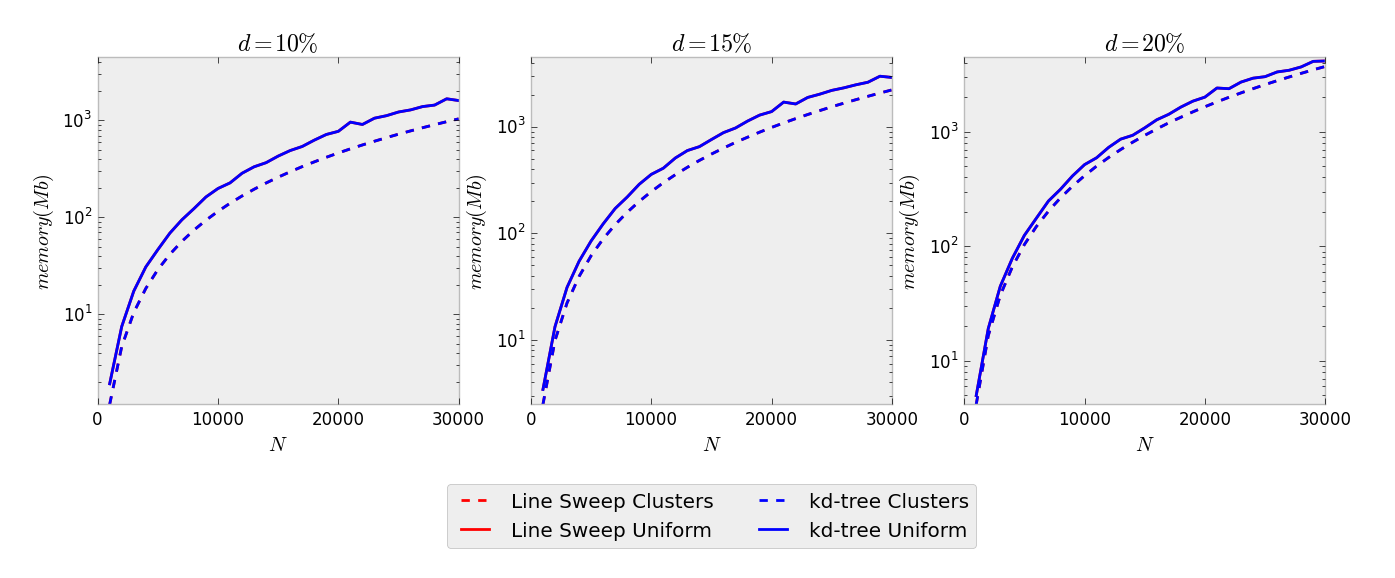
\includegraphics[width=\linewidth]{Pictures/ls_kd_s}
    \label{fig:ls_kd_s} 
\end{figure}


\begin{figure}[H] 
  \begin{subfigure}[b]{0.5\linewidth}
    \centering
    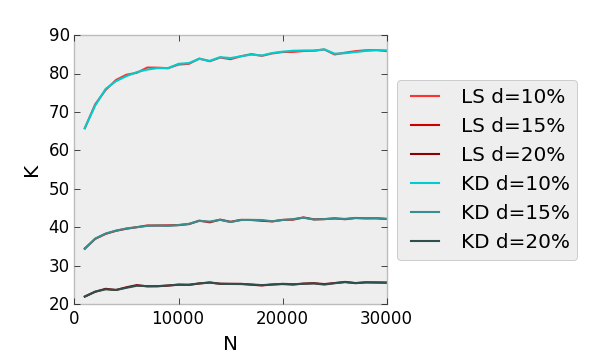
\includegraphics[width=0.9\linewidth]{Pictures/unif_kd_ls_k} 
    %\caption{$N=10$} 
    \label{fig:unif_kd_ls_k} 
    \vspace{4ex}
  \end{subfigure}%% 
  \begin{subfigure}[b]{0.5\linewidth}
    \centering
    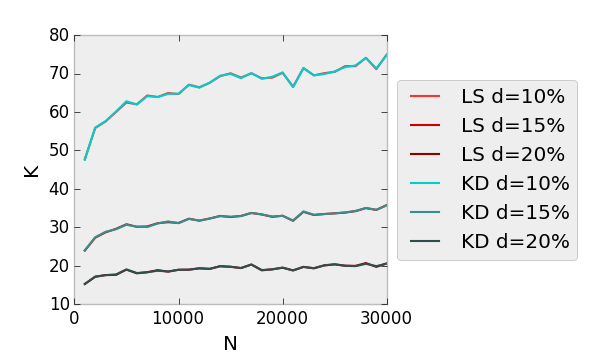
\includegraphics[width=0.9\linewidth]{Pictures/clus_kd_ls_k} 
    %\caption{$N=20$} 
    \label{fig:clus_kd_ls_k} 
    \vspace{4ex}
  \end{subfigure}
  \caption[Number $K$ of points selected for Line Sweep and $k$-d Tree range search]{Number $K$ of points selected for both proximity graph algorithms on uniform inputs(left) and clustered inputs(right).}
  \label{fig:kd_ls_k} 
\end{figure}



The process of finding the best disposition of circles of the same radius in a given area is known as circle packing. The number of circles in a circle packing instance for a square area is given by the ratio between the circles' radii and the width of the square enclosing them. Since the value for $d$ is given as a fraction of the size of the window, the bound values of $k$ can be calculated for the various values of $d$. A detailed explanation of how to calculate the values for the upper bound is given in Appendix \ref{ann:packing}. The values indicate that $k$ should not be larger than $\{128,59,36\}$, for the given values $d=\{0.1,0.15,0.2\}$, respectively. With the exception of the latter, these values are yet to be proven to be optimal, but are not expected to be very different, and serve as a good estimate of the maximum number of points that can be selected.

These results suggest that the best algorithm to use is the line sweep algorithm, as it takes less time and the same memory to compute similar results.
	
\section{Heuristic Speed-ups}
The approximation algorithm runs rather efficiently, taking under 1 second for 30000 points for the uniform inputs, and under 3 seconds for the clustered inputs. Nonetheless, they are very memory intensive, which could present an issue for larger instances. This result can be improved by employing some heuristic filtering methods to the inputs. By using these approaches, however, the guarantee of the quality of the approximation is lost. Nevertheless, the results may indicate if the heuristic algorithms should still be considered to handle larger numbers of points.

\subsection{Random Sampling}
The simplest method to speed-up the algorithms is to simply ignore a randomly chosen subset of those points. With the smaller sample of points, the algorithm should run faster and use less memory space. If the points are removed uniformly, then the overall distribution should still be kept. Two versions of this method were tested. In the first, only one in every five points was considered by the algorithm, whereas in the second only one in every ten were. Figure \ref{fig:ls_rs_t} shows the time difference between the regular line sweep and the randomly sampled input algorithms.
The graph proves that the sampling is indeed faster. This speed-up is caused by the lower number of starting points for the algorithm to process. 

The smaller number also affects the memory needed by these algorithms, which require less space to store the graph. This happens because the number of edges tends to grow quadratically in relation to the number of points, meaning that a set with $1/5$th of the points would be expected to have around $1/25$th of the edges. Figure \ref{fig:ls_rs_s} shows the space used by the programs. This time, no cases that exceeded the memory limit were recorded. The figure shows that the random samples use the space expected above. Where the line sweep algorithm uses an average of 4164.93Mb for the clustered inputs, the random samples use 167.83Mb for the $1/5$th sample version and 41.44Mb for the $1/10$ sample version. The uniform inputs had a similar result, with the line sweep algorithm using an average of 3729.71Mb for the largest inputs, and the random sample algorithms using 149.17Mb for the $1/5$th sample version and 37.31Mb in the $1/10$th sample version, matching our initial prediction of $1/25$th and $1/100$th the amount of memory used by the line sweep algorithm to the second decimal case. 

\begin{figure}[H] 
	\centering
	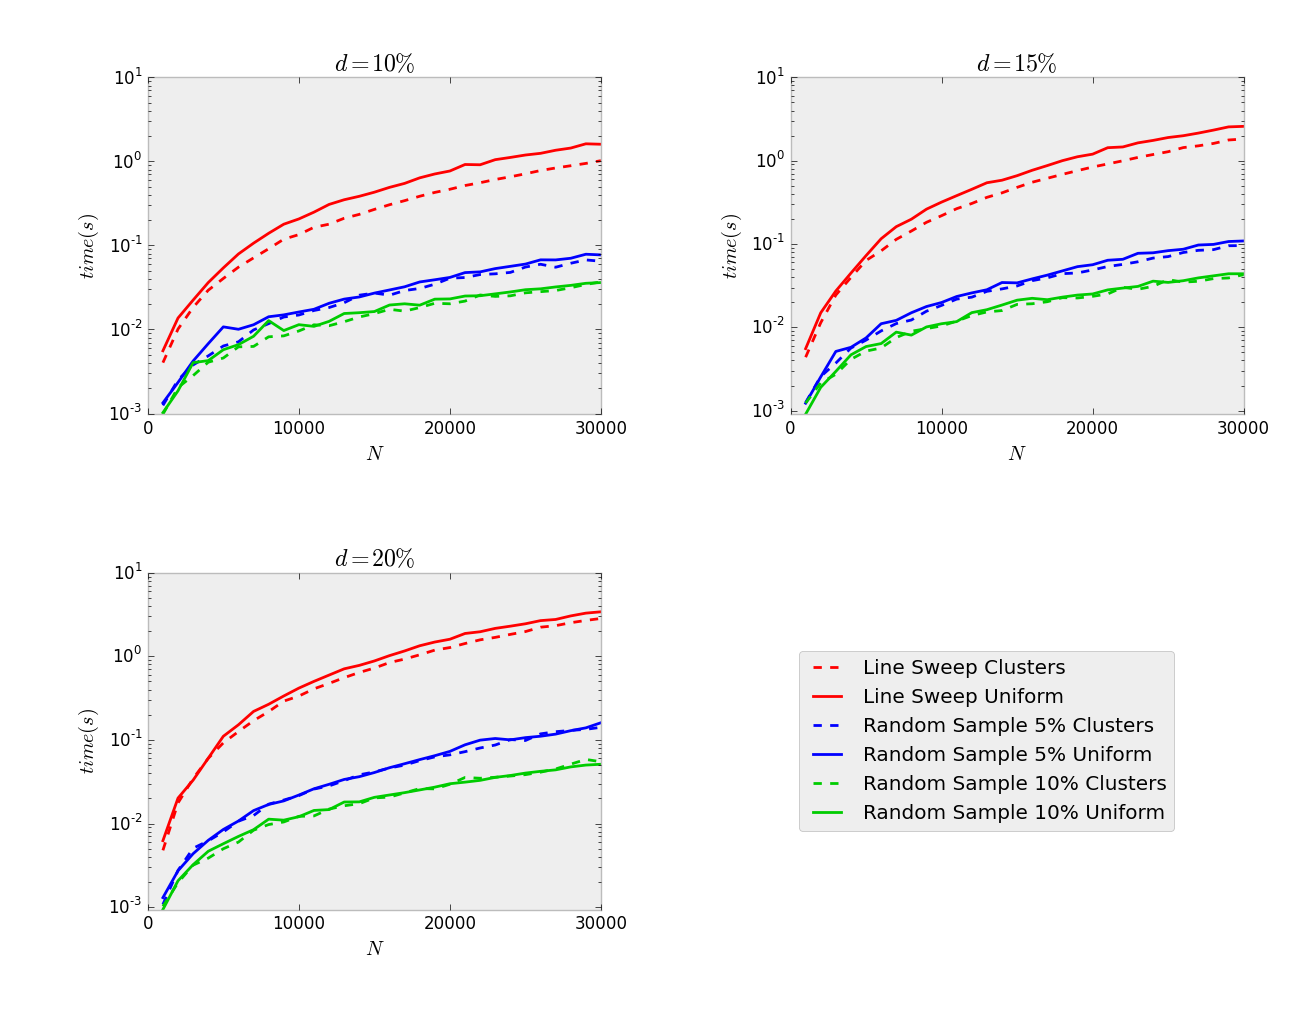
\includegraphics[width=0.8\linewidth]{Pictures/ls_rs_t} 
	\caption[CPU-time for Line Sweep and Random Sampling algorithms.]{CPU-time for the line sweep algorithm, and two instances of the random sampling, with 5\% and 10\% of the total points, for different values of $d$.}
	\label{fig:ls_rs_t} 
\end{figure}
\begin{figure}[!h] 
	\vspace{-10pt}
	\centering
	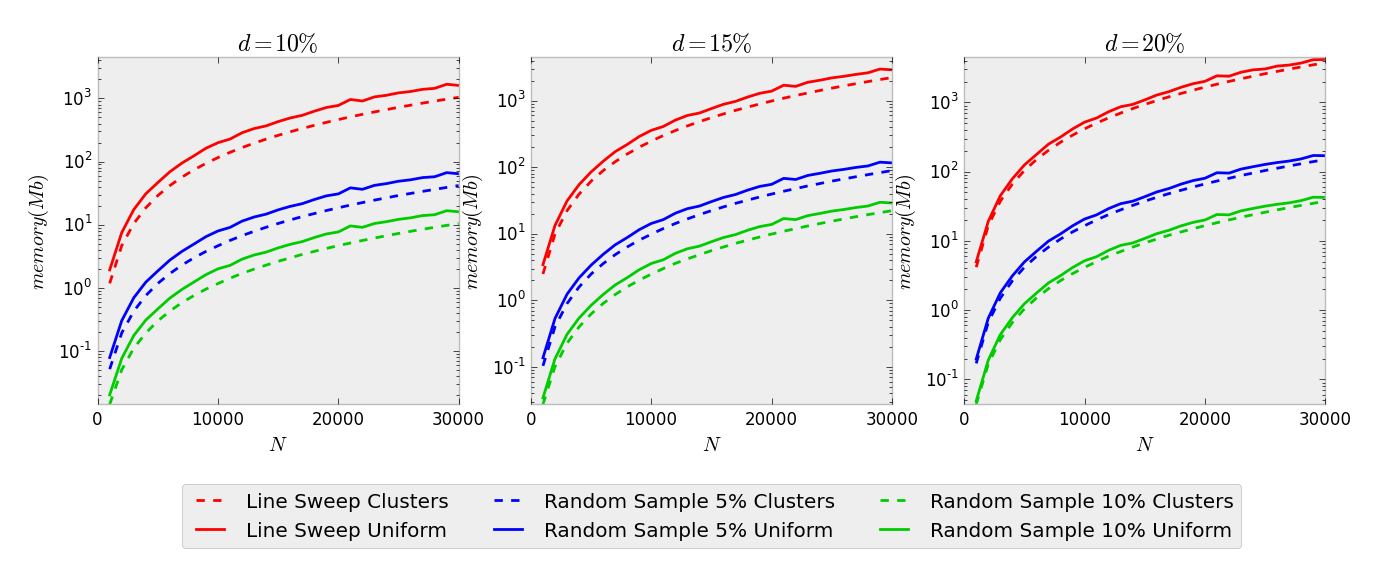
\includegraphics[width=\linewidth]{Pictures/ls_rs_s} 
	\label{fig:ls_rs_s} 
\end{figure}
\begin{figure}[H] 
  \begin{subfigure}[b]{0.5\linewidth}
    \centering
    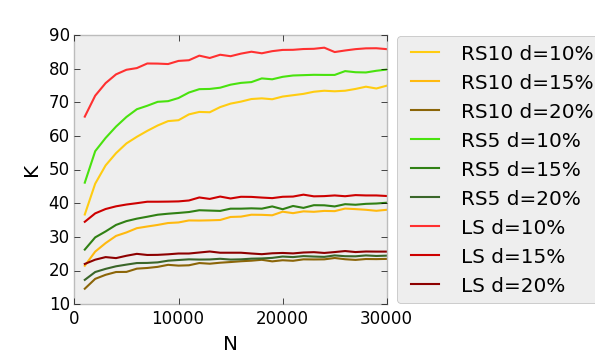
\includegraphics[width=0.9\linewidth]{Pictures/unif_ls_rs_k} 
    %\caption{$N=10$} 
    \label{fig:unif_ls_rs_k} 
    \vspace{4ex}
  \end{subfigure}%% 
  \begin{subfigure}[b]{0.5\linewidth}
    \centering
    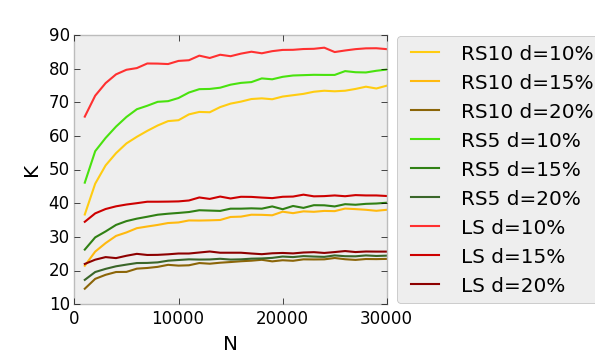
\includegraphics[width=0.9\linewidth]{Pictures/unif_ls_rs_k} 
    %\caption{$N=20$} 
    \label{fig:clus_ls_rs_k} 
    \vspace{4ex}
  \end{subfigure}
  \caption{Number $K$ of points selected for both random sample algorithms on uniform points(left) and clustered points (right). The red lines represent the control group (line sweep), the green lines represent the 1/5th sampling and the yellow lines represent the 1/10th sampling}
  \label{fig:ls_rs_k} 
\end{figure}



Upon closer inspection, however, it can be noted that the resulting set is not optimal. Figure \ref{fig:ls_rs_k} shows that the number of selected points is inferior.
This can be explained by the fact that the algorithm is not accounting for all points. In fact, whenever the original set has one isolated point, away from any other by more than the coverage distance, it has a 4 out of 5 chance of being discarded and unaccounted for (or 9 out of 10, depending on the version of the algorithm). This means that not all points are being covered, and the number of selected points decreases. Figure \ref{fig:ls_rs_greece} shows this effect in a real map.

\begin{figure}[!h] 
  \centering
  \begin{subfigure}[b]{0.45\linewidth}
    \centering
    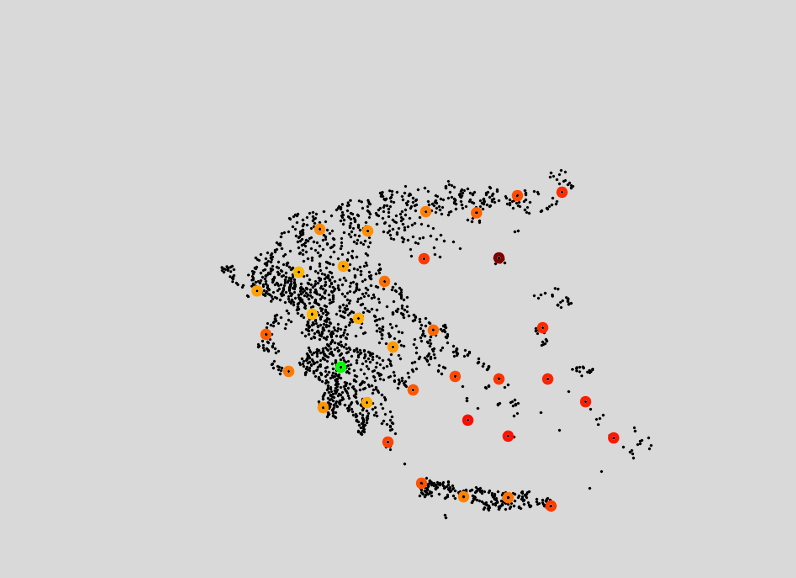
\includegraphics[width=0.9\linewidth]{Pictures/rs_greece} 
    %\caption{$N=10$} 
    \label{fig:ls_greece} 
  \end{subfigure}%% 
  \begin{subfigure}[b]{0.45\linewidth}
    \centering
    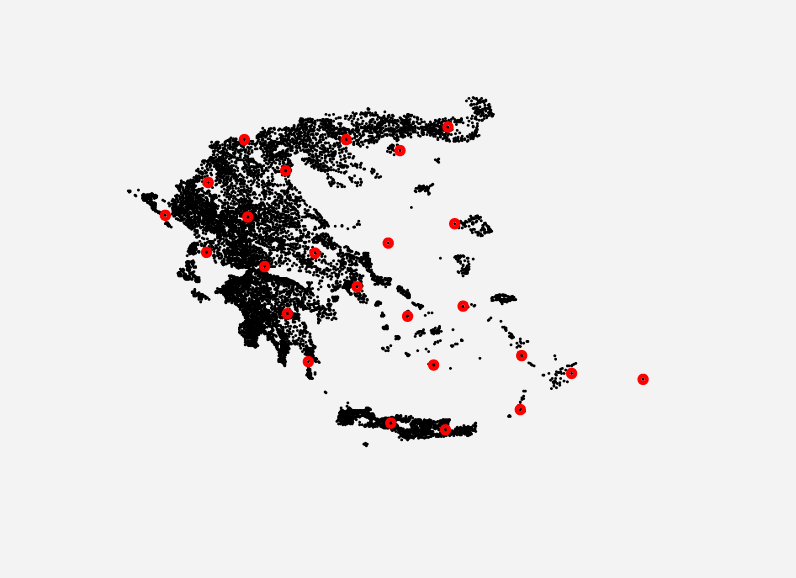
\includegraphics[width=0.9\linewidth]{Pictures/ls_greece} 
    %\caption{$N=20$} 
    \label{fig:rs_greece} 
  \end{subfigure}
  \label{fig:ls_rs_greece} 
\end{figure}



As shown, the sampled subset does not cover the most isolated points. In fact, the westernmost point in the map is not present in the sample and, therefore, is not covered. This method is not suitable for the initial requirements, since very isolated points have only a small chance of being represented.

\subsection{Two-phase filtering}

A solution tat avoids the flaws of the random sampling algorithm is to perform two passes of the approximation algorithm for the geometric disk cover problem. The first pass over the points is done with a very small radius $d^\prime$, since using a small distance speeds the algorithm up, as previously seen in Figure \ref{fig:ls_rs_t}. This can be done very quickly, since the range search only has to look in a very small area. This means that many of the points that are close to each other are discarded, but a representative neighbour is always left in its place. Isolated points are then never unaccounted for. The resulting set is much smaller than the original, whilst still keeping a representativeness degree. The second pass, now with the full coverage distance $d$ takes advantage of the much smaller set of points for the speed-up. 

Despite accounting for isolated points, the resulting set does not necessarily cover all the points with disks of radii $d$. Because the first pass transforms the set into disks of radii $d^\prime$, and the second pass only considers their centre point as the measure of cover, then there can be points that are further away from the centroids than $d$, the maximum distance being $d+d^\prime$, as shown in Figure \ref{fig:bp_error}. This means that by the strict definition of having all points covered by the disks, there are points left uncovered, but only by a guaranteed margin.

\begin{figure}[H]
\begin{center}
	
	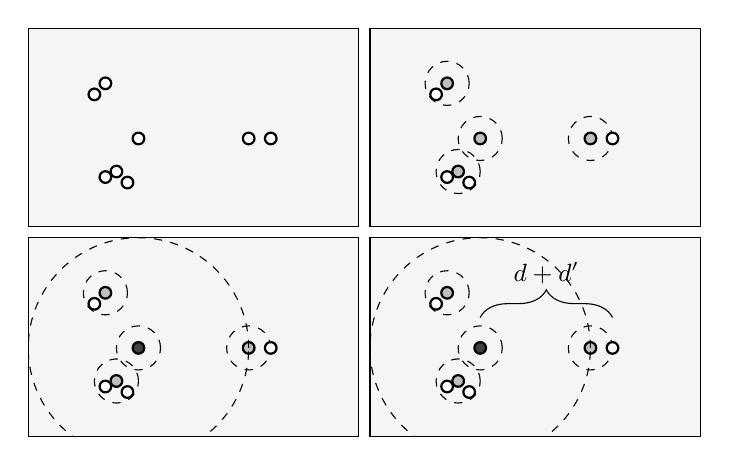
\begin{tikzpicture}[scale=1.4]
	\begin{scope}[]
	\fill[lightgray!15,draw=black] (-1,-0.8) rectangle (2,1);
	\fill[white,draw=black,thick] (0,0) circle (1.5pt);
	\fill[white,draw=black,thick] (1,0) circle (1.5pt);
	\fill[white,draw=black,thick] (1.2,0) circle (1.5pt);
	
	\fill[white,draw=black,thick] (-0.3,0.5) circle (1.5pt);
	\fill[white,draw=black,thick] (-0.4,0.4) circle (1.5pt);
	\fill[white,draw=black,thick] (-0.2,-0.3) circle (1.5pt);
	\fill[white,draw=black,thick] (-0.1,-0.4) circle (1.5pt);
	\fill[white,draw=black,thick] (-0.3,-0.35) circle (1.5pt);
	\end{scope}
	\begin{scope}[shift={(3.1,0)}]
	\fill[lightgray!15,draw=black] (-1,-0.8) rectangle (2,1);
	\fill[lightgray,draw=black,thick] (0,0) circle (1.5pt);
	\fill[lightgray,draw=black,thick] (1,0) circle (1.5pt);
	\fill[lightgray,draw=black,thick] (-0.2,-0.3) circle (1.5pt);
	\fill[lightgray,draw=black,thick] (-0.3,0.5) circle (1.5pt);
	
	\draw[dashed] (0,0) circle (0.2);
	\draw[dashed] (1,0) circle (0.2);
	\draw[dashed] (-0.2,-0.3) circle (0.2);
	\draw[dashed] (-0.3,0.5) circle (0.2);
	
	\fill[white,draw=black,thick] (1.2,0) circle (1.5pt);
	\fill[white,draw=black,thick] (-0.4,0.4) circle (1.5pt);
	\fill[white,draw=black,thick] (-0.1,-0.4) circle (1.5pt);
	\fill[white,draw=black,thick] (-0.3,-0.35) circle (1.5pt);
	\end{scope}
	\begin{scope}[shift={(0,-1.9)}]
	\fill[lightgray!15,draw=black] (-1,-0.8) rectangle (2,1);
	\clip (-1,-0.8) rectangle (2,1);
	
	\fill[darkgray,draw=black,thick] (0,0) circle (1.5pt);
	\fill[lightgray,draw=black,thick] (1,0) circle (1.5pt);
	\fill[lightgray,draw=black,thick] (-0.2,-0.3) circle (1.5pt);
	\fill[lightgray,draw=black,thick] (-0.3,0.5) circle (1.5pt);
	
	
	\draw[dashed] (0,0) circle (1);
	\draw[dashed] (0,0) circle (0.2);
	\draw[dashed] (1,0) circle (0.2);
	\draw[dashed] (-0.2,-0.3) circle (0.2);
	\draw[dashed] (-0.3,0.5) circle (0.2);
	
	\fill[white,draw=black,thick] (1.2,0) circle (1.5pt);
	\fill[white,draw=black,thick] (-0.4,0.4) circle (1.5pt);
	\fill[white,draw=black,thick] (-0.1,-0.4) circle (1.5pt);
	\fill[white,draw=black,thick] (-0.3,-0.35) circle (1.5pt);
	\end{scope}
	
	\begin{scope}[shift={(3.1,-1.9)}]
	\fill[lightgray!15,draw=black] (-1,-0.8) rectangle (2,1);
	\clip (-1,-0.8) rectangle (2,1);
	
	\fill[darkgray,draw=black,thick] (0,0) circle (1.5pt);
	\fill[lightgray,draw=black,thick] (1,0) circle (1.5pt);
	\fill[lightgray,draw=black,thick] (-0.2,-0.3) circle (1.5pt);
	\fill[lightgray,draw=black,thick] (-0.3,0.5) circle (1.5pt);
	
	
	\draw[dashed] (0,0) circle (1);
	\draw[dashed] (0,0) circle (0.2);
	\draw[dashed] (1,0) circle (0.2);
	\draw[dashed] (-0.2,-0.3) circle (0.2);
	\draw[dashed] (-0.3,0.5) circle (0.2);
	
	\fill[white,draw=black,thick] (1.2,0) circle (1.5pt);
	\fill[white,draw=black,thick] (-0.4,0.4) circle (1.5pt);
	\fill[white,draw=black,thick] (-0.1,-0.4) circle (1.5pt);
	\fill[white,draw=black,thick] (-0.3,-0.35) circle (1.5pt);
	
	
	\draw [decorate,decoration={brace,amplitude=10pt,mirror,raise=4pt},yshift=5pt]
	(1.2,0) -- (0,0) node [black,midway,yshift=20] {\small	$d+d'$};
	
	
	\end{scope}
	
	\end{tikzpicture}

\end{center}
\caption{Illustration of the worst case scenario for the error of the biphasic method}
\label{fig:bp_error}
\end{figure}


The \emph{CPU} times for three instances of the algorithm can be seen in Figure \ref{fig:ls_bp_t}. The values of the first pass distance $d^\prime$ are given as a percentage of the final pass distance $d$. One of the instances uses $d^\prime=0.05d$, another $d^\prime=0.1d$ and the other uses $d^\prime=0.2d$.

As it can be seen, the two-phase filtering is more efficient than the simple line sweep algorithm and does not seem to vary a lot with the total number of points. The first pass eliminates a very large number of redundant points, leaving a similar resulting set for different values of $N$. The intermediate subset is still representative of the original. 

The smaller distance requires less edges to be created, and the proximity graph for the first phase is uses less space than a one-phase algorithm does. The proximity graph for the second phase benefits from having less points, thus requiring less edges. Since this algorithm calculates two graphs, both of which sparser than the complete on in the Line Sweep and \kdtree algorithms, the memory limit was not an issue for the inputs tested. Figure \ref{fig:ls_bp_s} shows the memory footprint of the three versions of the algorithm. These algorithms are less predictable concerning the size of the graphs, since they depend a lot from local density of points for the first phase. While they do not have as small a footprint as the random sampling, they still use considerably less than the line sweep and \kdtree range search. 

These algorithms do not share the issue of leaving isolated points completely uncovered like the random sampling algorithms do, returning better representative subsets. Figure \ref{fig:ls_bp_k} shows the variation in size of the final subset chosen by the two-phase filtering algorithms.

The graph shows that despite the two-phase algorithms returning lower numbers of $K$, they are not as low as the random sampling. 

\begin{figure}[!h]  
	\vspace{-25pt}
	\centering
	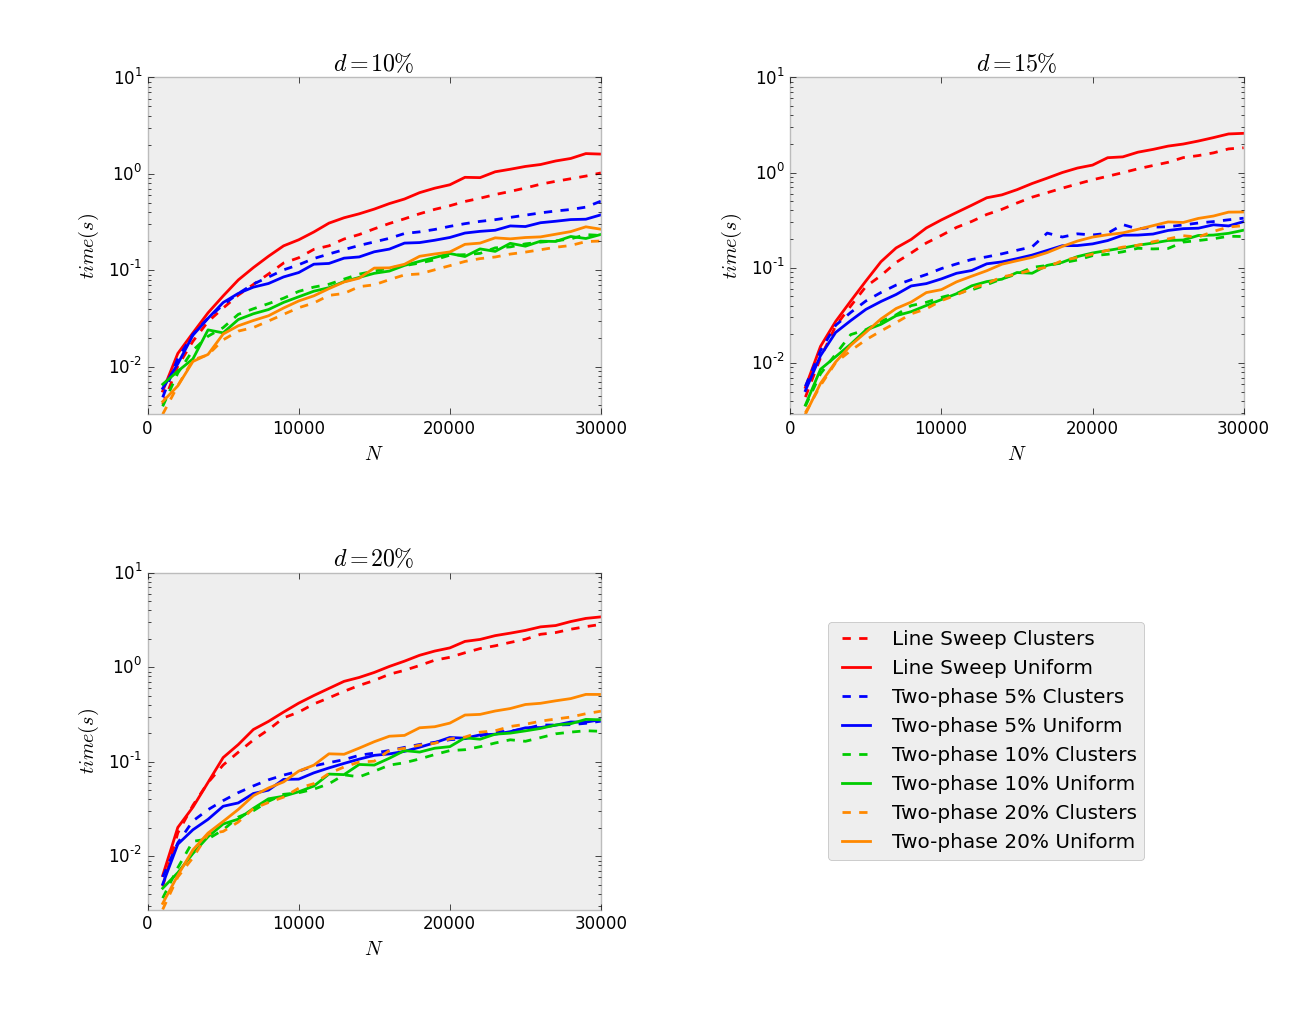
\includegraphics[width=\linewidth]{Pictures/ls_bp_t} 
	\label{fig:ls_bp_t} 
\end{figure}
\begin{figure}[!h]   
	\vspace{-10pt}
	\centering
	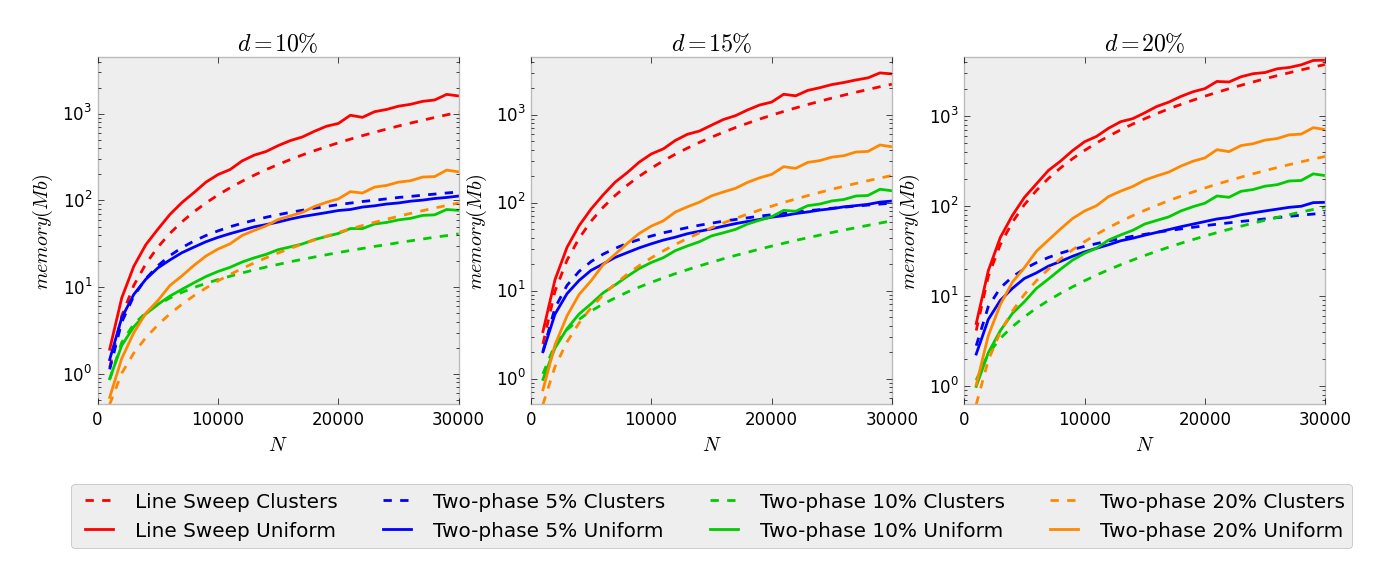
\includegraphics[width=\linewidth]{Pictures/ls_bp_s} 
	\caption[Memory used by Line Sweep and Two-phase filter algorithms..]{Memory used by the line sweep algorithm, and three instances of the Two-phase filter, with $d^\prime=5\%$, $d^\prime=10\%$ and $d^\prime=20\%$ in relation to $d$. Since two graphs are built, only the larger one is considered for this graph, as they are never simultaneously stored in memory.}
	\label{fig:ls_bp_s} 
\end{figure}
\begin{figure}[!h]   
	\vspace{-10pt}
	\centering
	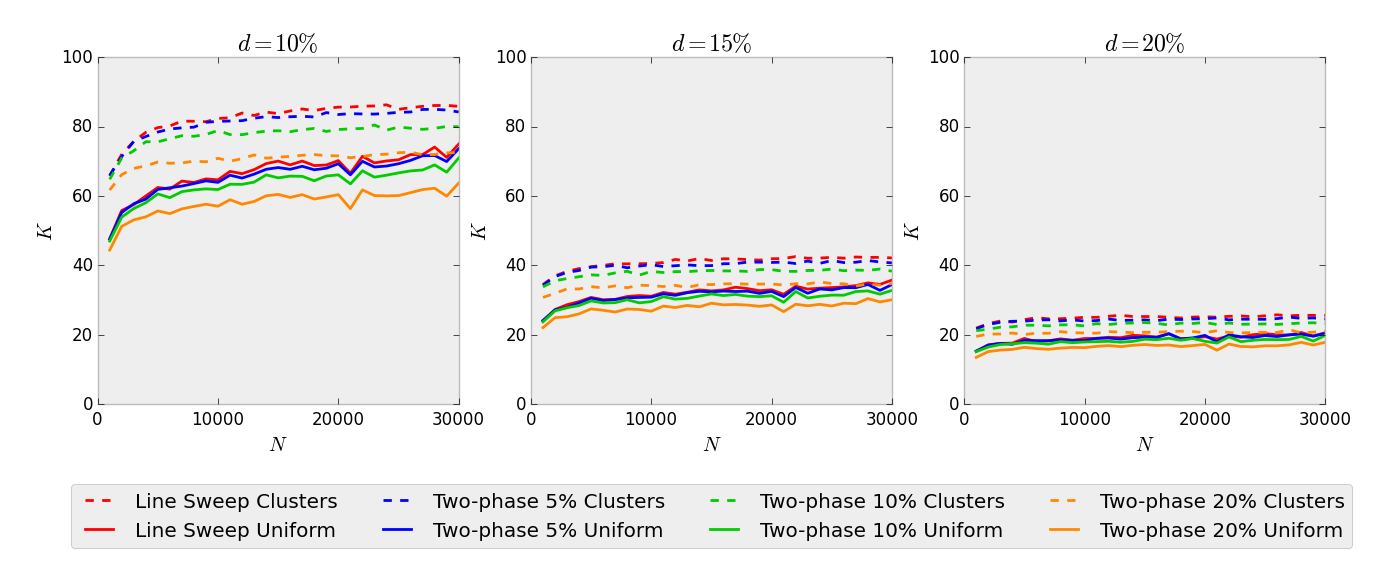
\includegraphics[width=\linewidth]{Pictures/ls_bp_k} 
	\label{fig:ls_bp_k} 
\end{figure}

This result has some effect on the quality, but it is not nearly as noticeable as the results from the random sampling. Figure \ref{fig:bp_sweden} shows the compared output between the original line sweep algorithm, and the different versions of the two-phase algorithm, as well as their intermediate phases.


This final result shows that the two-phase filter, especially with $d^\prime=0.1d$, can yield very approximate results at a fraction of the time and space, thus making a good candidate to use with inputs larger than the regular Line Sweep method can handle.

\begin{figure}[H]
	\begin{subfigure}[b]{1\linewidth}
		\centering
	\begin{subfigure}[t]{0.29\linewidth}
		\centering
		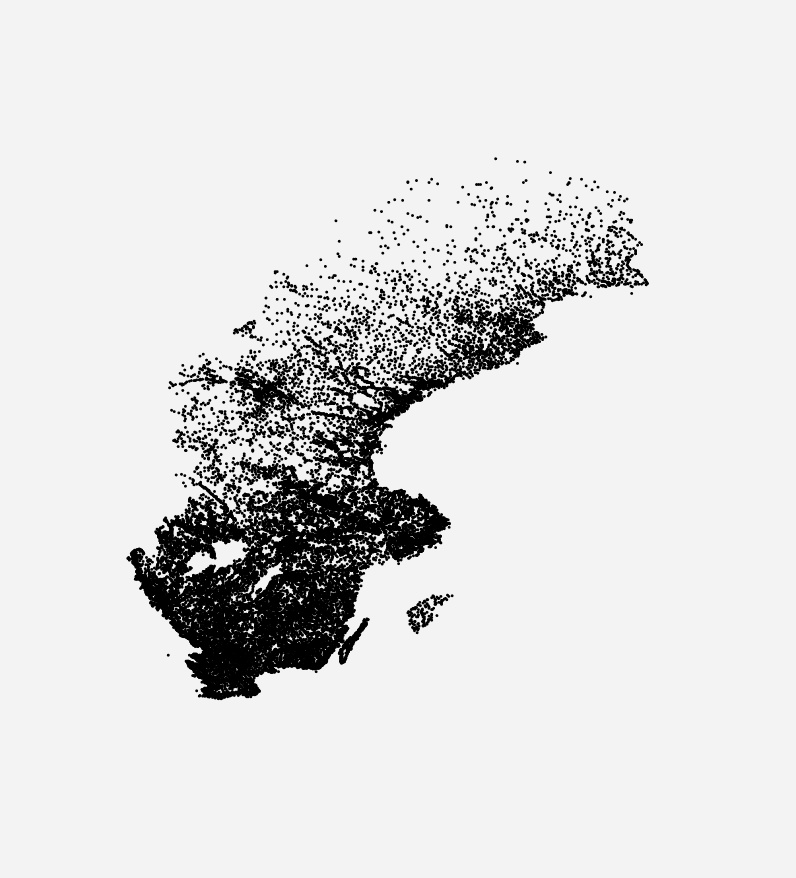
\includegraphics[width=0.9\linewidth]{Pictures/sweden} 
		\caption{} 
		\label{fig:sweden2} 
		\vspace{4ex}
	\end{subfigure}%% 
	\begin{subfigure}[t]{0.29\linewidth}
		\centering
		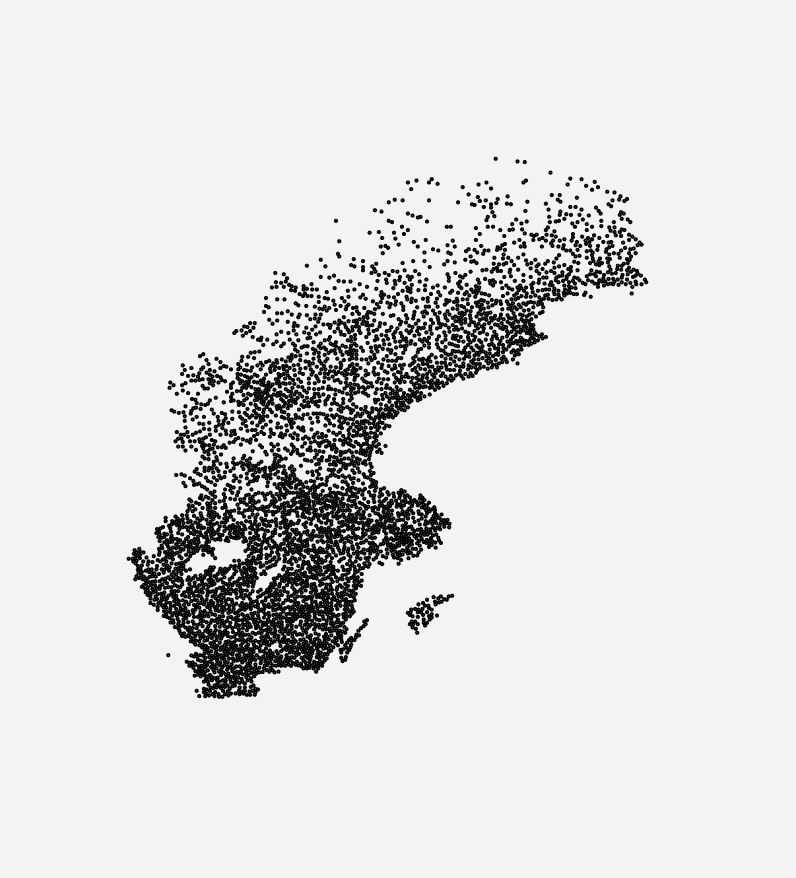
\includegraphics[width=0.9\linewidth]{Pictures/bp5_1_sweden} 
		\caption{} 
		\label{fig:bp5_1_sweden} 
		\vspace{4ex}
	\end{subfigure}
	\begin{subfigure}[t]{0.29\linewidth}
		\centering
		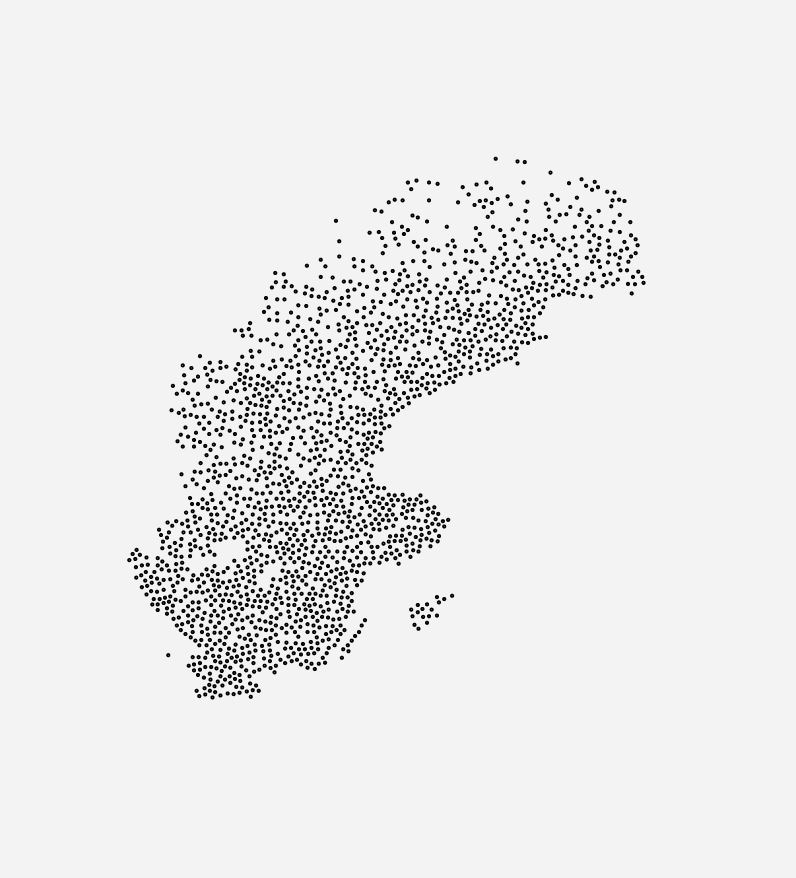
\includegraphics[width=0.9\linewidth]{Pictures/bp10_1_sweden}
		\caption{} 
		\label{fig:bp10_1_sweden} 
		\vspace{4ex}
	\end{subfigure}
\end{subfigure}
\begin{subfigure}[b]{1\linewidth}
	\centering
  \begin{subfigure}[b]{0.29\linewidth}
  	\centering
  	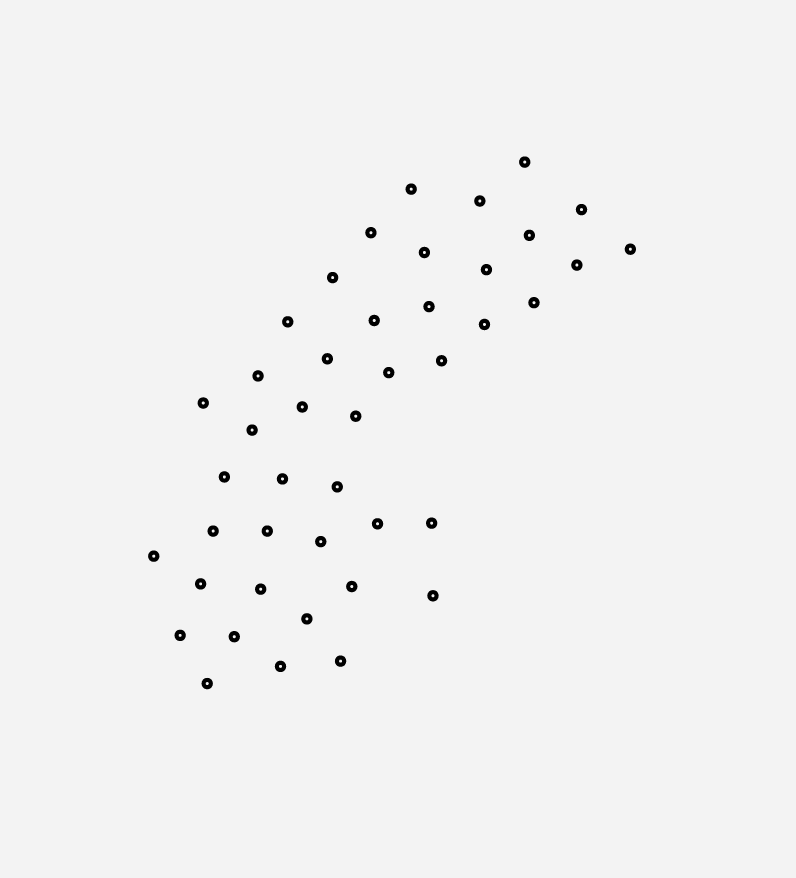
\includegraphics[width=0.9\linewidth]{Pictures/ls_10_sweden} 
  	\caption{} 
  	\label{fig:ls_10_sweden2} 
  	\vspace{4ex}
  \end{subfigure}%% 
  \begin{subfigure}[b]{0.29\linewidth}
  	\centering
  	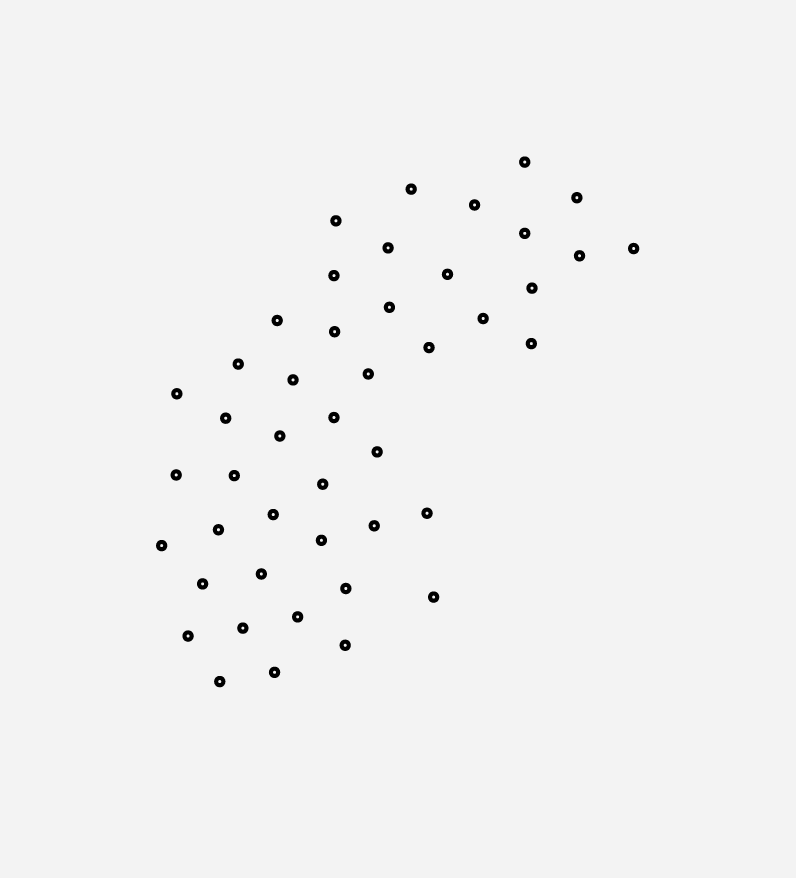
\includegraphics[width=0.9\linewidth]{Pictures/bp5_2_sweden} 
  	\caption{} 
  	\label{fig:bp5_2_sweden} 
  	\vspace{4ex}
  \end{subfigure}
  \begin{subfigure}[b]{0.29\linewidth}
  	\centering
  	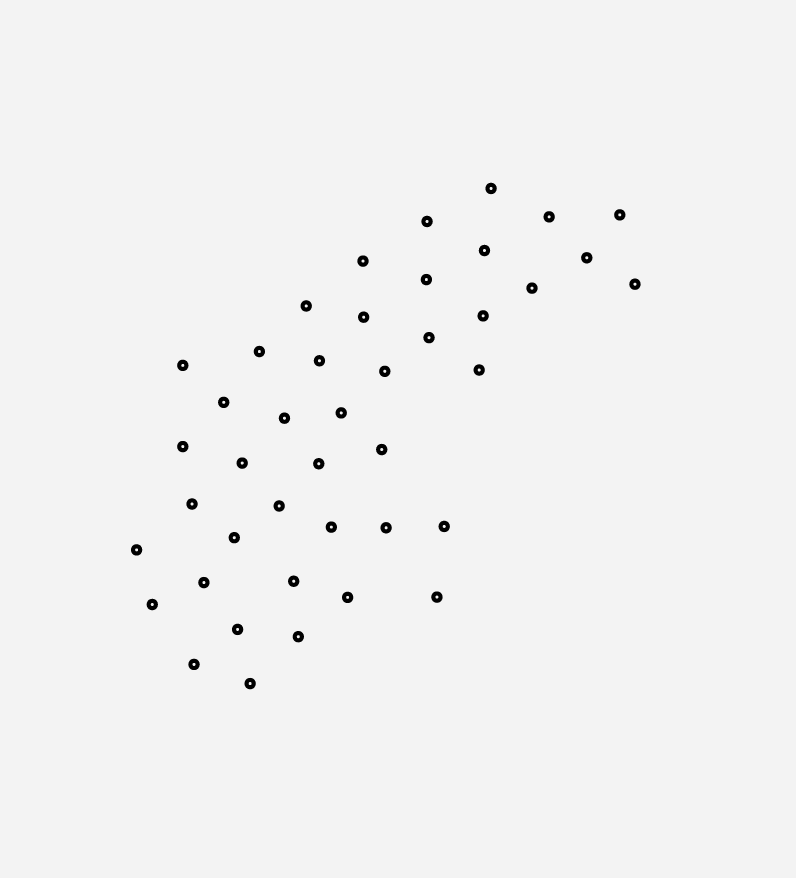
\includegraphics[width=0.9\linewidth]{Pictures/bp10_2_sweden} 
  	\caption{} 
  	\label{fig:bp10_2_sweden} 
  	\vspace{4ex}
  \end{subfigure}
\end{subfigure}
  \caption{Biphasic Filter result comparison.}
  \centering \small
  \parbox{0.5\linewidth}{(A) Original Set (B) Intermediate Set for Biphasic Filter with $d'=0.05d$ (C) Intermediate Set for Biphasic Filter with $d'=0.1d$ (D) Final Set for one pass (E) Final Set for Biphasic Filter with $d'=0.05d$ (F) Final Set for Biphasic Filter with $d'=0.1d$ }
  \label{fig:bp_sweden} 
\end{figure}



\section{Region Panning and Zooming}
One of the requirements established for the final algorithm it that it should be able to handle a translation motion in the region and starting point set. This means that in case the new region intersects the previous one, it is important for the user that the points already in display are kept selected, so that each move does not cause the user to lose track of the movement. As such, any selected centroids inside the intersection of the two regions, and all the points covered by them, should be kept unchanged, even if it means losing the guaranteed approximation to the optimal value. Each of the approaches described earlier can be modified to ensure that this property is met. 

To handle the panning case, each instance of the program receives the centroids chosen in the previous region. To ensure that the points are still selected is a matter of artificially increasing their number of neighbours by $N$, then compute the problem regularly.  Since the number of points from the old region is bound from above by at most 128, the new number of points is relatively insignificant for instances of 10000 points and more, and the algorithms show no significant difference in performance. Since the covering distance does not change, the old centroids are not close enough together to cover each other, otherwise they would have done so in the old region. This solves the panning issue without needing to add much complexity to the algorithms. In the case of multiple phase filters, the weight of the selected points must be artificially increased in all the phases, to ensure they are kept selected.

\begin{figure}[!h]
	\centering	
	\begin{tikzpicture}[scale=0.35]
	\fill[lightgray!15,draw=black,thick] (0,0) rectangle (20,15);
	
	\fill[gray] (7.189873,12.007256) circle (3pt);
	\fill[gray] (1.032745,3.725546) circle (3pt);
	\fill[gray] (5.703827,13.261152) circle (3pt);
	\fill[gray] (17.936429,1.025270) circle (3pt);
	\fill[gray] (13.690591,3.939102) circle (3pt);
	\fill[gray] (11.193998,5.283551) circle (3pt);
	\fill[gray] (4.798022,11.213652) circle (3pt);
	\fill[gray] (18.715176,13.688003) circle (3pt);
	\fill[gray] (10.692704,11.860352) circle (3pt);
	\fill[gray] (7.056115,11.346718) circle (3pt);
	\fill[gray] (0.966585,7.071031) circle (3pt);
	\fill[gray] (13.937926,10.633255) circle (3pt);
	\fill[gray] (7.593829,6.185742) circle (3pt);
	\fill[gray] (3.705931,12.388078) circle (3pt);
	\fill[gray] (10.775614,14.295963) circle (3pt);
	\fill[gray] (18.057741,8.744112) circle (3pt);
	\fill[gray] (8.068603,12.323568) circle (3pt);
	\fill[gray] (18.650144,3.881699) circle (3pt);
	\fill[gray] (12.484510,6.800151) circle (3pt);
	\fill[gray] (13.183608,4.794407) circle (3pt);
	\fill[gray] (12.174938,11.920051) circle (3pt);
	\fill[gray] (1.736886,14.482144) circle (3pt);
	\fill[gray] (3.355545,10.638588) circle (3pt);
	\fill[gray] (0.295411,13.134745) circle (3pt);
	\fill[gray] (17.430353,3.016958) circle (3pt);
	\fill[gray] (19.869400,14.962442) circle (3pt);
	\fill[gray] (10.729442,1.767601) circle (3pt);
	\fill[gray] (0.984080,12.412868) circle (3pt);
	\fill[gray] (0.656211,2.050832) circle (3pt);
	\fill[gray] (6.149162,12.226380) circle (3pt);
	\fill[gray] (10.443128,14.550410) circle (3pt);
	\fill[gray] (18.655995,12.951857) circle (3pt);
	\fill[gray] (11.590530,9.448236) circle (3pt);
	\fill[gray] (7.243261,7.388230) circle (3pt);
	\fill[gray] (18.260829,1.052094) circle (3pt);
	\fill[gray] (9.825389,2.467039) circle (3pt);
	\fill[gray] (1.270561,12.927529) circle (3pt);
	\fill[gray] (2.183670,7.471334) circle (3pt);
	\fill[gray] (9.101712,4.988481) circle (3pt);
	\fill[gray] (2.138719,0.055549) circle (3pt);
	\fill[gray] (6.399133,11.770019) circle (3pt);
	\fill[gray] (16.541260,8.003890) circle (3pt);
	\fill[gray] (11.256169,10.807615) circle (3pt);
	\fill[gray] (17.926257,7.283852) circle (3pt);
	\fill[gray] (2.739774,2.765903) circle (3pt);
	\fill[gray] (18.966992,13.637273) circle (3pt);
	\fill[gray] (10.668147,0.016967) circle (3pt);
	\fill[gray] (0.310205,6.564354) circle (3pt);
	\fill[gray] (12.811328,2.473994) circle (3pt);
	\fill[gray] (11.566809,13.614052) circle (3pt);
	\fill[gray] (3.283881,1.735554) circle (3pt);
	\fill[gray] (14.101612,9.963662) circle (3pt);
	\fill[gray] (4.039885,7.059605) circle (3pt);
	\fill[gray] (16.591664,9.866772) circle (3pt);
	\fill[gray] (14.517395,8.977751) circle (3pt);
	\fill[gray] (10.426222,8.104159) circle (3pt);
	\fill[gray] (3.549166,4.048136) circle (3pt);
	\fill[gray] (17.483642,9.263434) circle (3pt);
	\fill[gray] (16.325371,10.266466) circle (3pt);
	\fill[gray] (10.979845,9.152594) circle (3pt);
	\fill[gray] (5.981012,10.220922) circle (3pt);
	\fill[gray] (13.465983,3.443126) circle (3pt);
	\fill[gray] (6.251647,7.884290) circle (3pt);
	\fill[gray] (4.363000,8.528955) circle (3pt);
	\fill[gray] (11.463047,7.570383) circle (3pt);
	\fill[gray] (6.761937,4.878485) circle (3pt);
	\fill[gray] (12.392466,2.219189) circle (3pt);
	\fill[gray] (15.739529,10.876258) circle (3pt);
	\fill[gray] (11.362909,4.028322) circle (3pt);
	\fill[gray] (1.403271,8.917787) circle (3pt);
	\fill[gray] (1.694522,9.344248) circle (3pt);
	\fill[gray] (4.738868,8.295962) circle (3pt);
	\fill[gray] (6.389808,9.547780) circle (3pt);
	\fill[gray] (8.886094,13.840983) circle (3pt);
	\fill[gray] (7.040599,4.696280) circle (3pt);
	\fill[gray] (14.952140,13.942108) circle (3pt);
	\fill[gray] (17.211416,0.139226) circle (3pt);
	\fill[gray] (10.670952,8.112072) circle (3pt);
	\fill[gray] (9.839079,10.382850) circle (3pt);
	\fill[gray] (16.809571,8.160259) circle (3pt);
	\fill[gray] (17.478862,13.197850) circle (3pt);
	\fill[gray] (16.008395,0.995887) circle (3pt);
	\fill[gray] (6.135184,1.721209) circle (3pt);
	\fill[gray] (7.202958,11.088303) circle (3pt);
	\fill[gray] (15.604905,3.537251) circle (3pt);
	\fill[gray] (4.649788,5.960632) circle (3pt);
	\fill[gray] (12.646831,1.748152) circle (3pt);
	\fill[gray] (5.704931,3.385258) circle (3pt);
	\fill[gray] (13.244499,4.627266) circle (3pt);
	\fill[gray] (13.866541,3.042211) circle (3pt);
	\fill[gray] (4.020821,13.829378) circle (3pt);
	\fill[gray] (14.478915,3.303659) circle (3pt);
	\fill[gray] (12.119582,8.071522) circle (3pt);
	\fill[gray] (0.052974,5.544991) circle (3pt);
	\fill[gray] (14.157844,2.072198) circle (3pt);
	\fill[gray] (19.829076,4.945795) circle (3pt);
	\fill[gray] (19.464476,12.758033) circle (3pt);
	\fill[gray] (14.448449,14.224297) circle (3pt);
	\fill[gray] (8.325068,2.544047) circle (3pt);
	\fill[gray] (4.359520,7.930448) circle (3pt);
	\fill[gray] (3.633524,14.815104) circle (3pt);
	\fill[gray] (17.042602,3.044707) circle (3pt);
	\fill[gray] (11.717216,4.551330) circle (3pt);
	\fill[gray] (0.494682,8.633230) circle (3pt);
	\fill[gray] (13.979299,5.732816) circle (3pt);
	\fill[gray] (18.535276,6.350147) circle (3pt);
	\fill[gray] (8.267637,9.654893) circle (3pt);
	\fill[gray] (0.880287,7.026485) circle (3pt);
	\fill[gray] (7.695881,2.684383) circle (3pt);
	\fill[gray] (2.465090,8.505883) circle (3pt);
	\fill[gray] (14.415714,1.302376) circle (3pt);
	\fill[gray] (15.569702,0.753946) circle (3pt);
	\fill[gray] (18.285254,14.497479) circle (3pt);
	\fill[gray] (0.455887,6.378918) circle (3pt);
	\fill[gray] (12.197111,14.685628) circle (3pt);
	\fill[gray] (6.795592,4.486260) circle (3pt);
	\fill[gray] (16.686419,3.579784) circle (3pt);
	\fill[gray] (3.510219,9.522966) circle (3pt);
	\fill[gray] (6.822231,1.872439) circle (3pt);
	\fill[gray] (1.037286,8.323394) circle (3pt);
	\fill[gray] (18.556981,12.076557) circle (3pt);
	\fill[gray] (3.117391,6.651586) circle (3pt);
	\fill[gray] (13.304852,5.408005) circle (3pt);
	\fill[gray] (2.023153,13.521868) circle (3pt);
	\fill[gray] (2.147448,11.752045) circle (3pt);
	\fill[gray] (9.632847,4.159554) circle (3pt);
	\fill[gray] (2.012655,11.451130) circle (3pt);
	\fill[gray] (19.605825,11.716914) circle (3pt);
	\fill[gray] (10.634260,5.094222) circle (3pt);
	\fill[gray] (4.929862,4.234030) circle (3pt);
	\fill[gray] (11.779346,12.733778) circle (3pt);
	\fill[gray] (17.355771,7.671409) circle (3pt);
	\fill[gray] (16.264088,11.902180) circle (3pt);
	\fill[gray] (0.851292,4.229110) circle (3pt);
	\fill[gray] (14.911070,2.246137) circle (3pt);
	\fill[gray] (12.790055,3.240956) circle (3pt);
	\fill[gray] (3.106337,9.853823) circle (3pt);
	\fill[gray] (15.004812,12.957114) circle (3pt);
	\fill[gray] (11.455350,11.640517) circle (3pt);
	\fill[gray] (16.862233,8.176758) circle (3pt);
	\fill[gray] (7.283005,1.511903) circle (3pt);
	\fill[gray] (14.023672,7.183187) circle (3pt);
	\fill[gray] (16.959859,4.239292) circle (3pt);
	\fill[gray] (9.080443,7.321678) circle (3pt);
	\fill[gray] (0.787920,14.235724) circle (3pt);
	\fill[gray] (9.757357,7.711644) circle (3pt);
	\fill[gray] (12.801919,8.156807) circle (3pt);
	\fill[gray] (19.173654,8.365171) circle (3pt);
	\fill[gray] (14.746939,5.266785) circle (3pt);
	\fill[gray] (15.460890,13.675672) circle (3pt);
	\fill[gray] (0.558498,1.426722) circle (3pt);
	\fill[gray] (5.319326,13.573341) circle (3pt);
	\fill[gray] (1.596066,12.682471) circle (3pt);
	\fill[gray] (10.411521,11.148780) circle (3pt);
	\fill[gray] (15.234786,12.617005) circle (3pt);
	\fill[gray] (0.878152,2.643967) circle (3pt);
	\fill[gray] (2.952409,6.694919) circle (3pt);
	\fill[gray] (9.074063,6.740000) circle (3pt);
	\fill[gray] (15.540580,11.468732) circle (3pt);
	\fill[gray] (18.001669,14.926523) circle (3pt);
	\fill[gray] (19.206391,12.660252) circle (3pt);
	\fill[gray] (13.006573,6.651786) circle (3pt);
	\fill[gray] (1.513548,14.283169) circle (3pt);
	\fill[gray] (7.830906,6.044319) circle (3pt);
	\fill[gray] (18.668757,5.840355) circle (3pt);
	\fill[gray] (12.281253,5.082468) circle (3pt);
	\fill[gray] (16.780682,6.387540) circle (3pt);
	\fill[gray] (11.968683,0.711781) circle (3pt);
	\fill[gray] (6.788235,8.014438) circle (3pt);
	\fill[gray] (0.289549,4.087150) circle (3pt);
	\fill[gray] (12.971851,6.048889) circle (3pt);
	\fill[gray] (3.067813,9.033496) circle (3pt);
	\fill[gray] (5.068369,9.124380) circle (3pt);
	\fill[gray] (5.587748,0.003656) circle (3pt);
	\fill[gray] (13.586570,4.533691) circle (3pt);
	\fill[gray] (6.431809,1.813709) circle (3pt);
	\fill[gray] (0.119261,12.849029) circle (3pt);
	\fill[gray] (11.383318,13.725656) circle (3pt);
	\fill[gray] (3.075973,13.633286) circle (3pt);
	\fill[gray] (8.271872,7.982950) circle (3pt);
	\fill[gray] (9.259674,2.953089) circle (3pt);
	\fill[gray] (9.308203,12.753614) circle (3pt);
	\fill[gray] (1.923948,7.874574) circle (3pt);
	\fill[gray] (10.934866,3.180220) circle (3pt);
	\fill[gray] (19.138825,13.620963) circle (3pt);
	\fill[gray] (7.627648,6.481897) circle (3pt);
	\fill[gray] (19.180860,1.683719) circle (3pt);
	\fill[gray] (8.589508,4.571152) circle (3pt);
	\fill[gray] (7.168202,8.919764) circle (3pt);
	\fill[gray] (17.585780,9.683140) circle (3pt);
	\fill[gray] (10.985187,8.586106) circle (3pt);
	\fill[gray] (8.981215,11.553663) circle (3pt);
	\fill[gray] (11.481412,5.212075) circle (3pt);
	\fill[gray] (19.557651,13.170481) circle (3pt);
	\fill[gray] (1.779307,9.969640) circle (3pt);
	\fill[gray] (19.033129,3.905117) circle (3pt);
	\fill[gray] (1.050651,10.469207) circle (3pt);
	\fill[gray] (2.370389,7.496352) circle (3pt);
	\fill[gray] (6.988479,11.647790) circle (3pt);
	\fill[gray] (5.818615,0.357924) circle (3pt);
	
	\draw[black,thick] (2,2) rectangle (13,9);
	\draw[black,thick,dashed] (7,5) rectangle (18,12);
	\draw[->,>=angle 60,black] (3,8) --(8,11);
	\draw[->,>=angle 60,black] (12,3) -- (17,6);
	\node at (3,3) {\large $A$};
	\node at (17,11) {\large $B$};
	
	\end{tikzpicture}
	\caption[Example of a panning motion]{Example of a panning motion from region $A$ to region $B$. Centroids contained in $A \cap B$ calculated in region $A$ must be kept when calculating region $B$.}
	\label{fig:panning}
\end{figure}

In the case of zooming, the scale changes, and so does the minimum distance. The points selected previously are relatively more close together in the new window, and they shift towards the centre of the region. One of the solutions is to simply discard the previous selected points, since they do not have the same representation properties they did in the previous region. Another solution is to do the same process as for the panning. By artificially inflating the weight of the established points, they are given priority over the new window's points. Since the points are now closer together in the window, they may cover each other, resulting in some prioritised points not being selected. 

\begin{figure}[!h]
	\centering
\begin{tikzpicture}[scale=0.35]
\fill[lightgray!15,draw=black,thick] (0,0) rectangle (20,15);

\fill[gray] (7.189873,12.007256) circle (3pt);
\fill[gray] (1.032745,3.725546) circle (3pt);
\fill[gray] (5.703827,13.261152) circle (3pt);
\fill[gray] (17.936429,1.025270) circle (3pt);
\fill[gray] (13.690591,3.939102) circle (3pt);
\fill[gray] (11.193998,5.283551) circle (3pt);
\fill[gray] (4.798022,11.213652) circle (3pt);
\fill[gray] (18.715176,13.688003) circle (3pt);
\fill[gray] (10.692704,11.860352) circle (3pt);
\fill[gray] (7.056115,11.346718) circle (3pt);
\fill[gray] (0.966585,7.071031) circle (3pt);
\fill[gray] (13.937926,10.633255) circle (3pt);
\fill[gray] (7.593829,6.185742) circle (3pt);
\fill[gray] (3.705931,12.388078) circle (3pt);
\fill[gray] (10.775614,14.295963) circle (3pt);
\fill[gray] (18.057741,8.744112) circle (3pt);
\fill[gray] (8.068603,12.323568) circle (3pt);
\fill[gray] (18.650144,3.881699) circle (3pt);
\fill[gray] (12.484510,6.800151) circle (3pt);
\fill[gray] (13.183608,4.794407) circle (3pt);
\fill[gray] (12.174938,11.920051) circle (3pt);
\fill[gray] (1.736886,14.482144) circle (3pt);
\fill[gray] (3.355545,10.638588) circle (3pt);
\fill[gray] (0.295411,13.134745) circle (3pt);
\fill[gray] (17.430353,3.016958) circle (3pt);
\fill[gray] (19.869400,14.962442) circle (3pt);
\fill[gray] (10.729442,1.767601) circle (3pt);
\fill[gray] (0.984080,12.412868) circle (3pt);
\fill[gray] (0.656211,2.050832) circle (3pt);
\fill[gray] (6.149162,12.226380) circle (3pt);
\fill[gray] (10.443128,14.550410) circle (3pt);
\fill[gray] (18.655995,12.951857) circle (3pt);
\fill[gray] (11.590530,9.448236) circle (3pt);
\fill[gray] (7.243261,7.388230) circle (3pt);
\fill[gray] (18.260829,1.052094) circle (3pt);
\fill[gray] (9.825389,2.467039) circle (3pt);
\fill[gray] (1.270561,12.927529) circle (3pt);
\fill[gray] (2.183670,7.471334) circle (3pt);
\fill[gray] (9.101712,4.988481) circle (3pt);
\fill[gray] (2.138719,0.055549) circle (3pt);
\fill[gray] (6.399133,11.770019) circle (3pt);
\fill[gray] (16.541260,8.003890) circle (3pt);
\fill[gray] (11.256169,10.807615) circle (3pt);
\fill[gray] (17.926257,7.283852) circle (3pt);
\fill[gray] (2.739774,2.765903) circle (3pt);
\fill[gray] (18.966992,13.637273) circle (3pt);
\fill[gray] (10.668147,0.016967) circle (3pt);
\fill[gray] (0.310205,6.564354) circle (3pt);
\fill[gray] (12.811328,2.473994) circle (3pt);
\fill[gray] (11.566809,13.614052) circle (3pt);
\fill[gray] (3.283881,1.735554) circle (3pt);
\fill[gray] (14.101612,9.963662) circle (3pt);
\fill[gray] (4.039885,7.059605) circle (3pt);
\fill[gray] (16.591664,9.866772) circle (3pt);
\fill[gray] (14.517395,8.977751) circle (3pt);
\fill[gray] (10.426222,8.104159) circle (3pt);
\fill[gray] (3.549166,4.048136) circle (3pt);
\fill[gray] (17.483642,9.263434) circle (3pt);
\fill[gray] (16.325371,10.266466) circle (3pt);
\fill[gray] (10.979845,9.152594) circle (3pt);
\fill[gray] (5.981012,10.220922) circle (3pt);
\fill[gray] (13.465983,3.443126) circle (3pt);
\fill[gray] (6.251647,7.884290) circle (3pt);
\fill[gray] (4.363000,8.528955) circle (3pt);
\fill[gray] (11.463047,7.570383) circle (3pt);
\fill[gray] (6.761937,4.878485) circle (3pt);
\fill[gray] (12.392466,2.219189) circle (3pt);
\fill[gray] (15.739529,10.876258) circle (3pt);
\fill[gray] (11.362909,4.028322) circle (3pt);
\fill[gray] (1.403271,8.917787) circle (3pt);
\fill[gray] (1.694522,9.344248) circle (3pt);
\fill[gray] (4.738868,8.295962) circle (3pt);
\fill[gray] (6.389808,9.547780) circle (3pt);
\fill[gray] (8.886094,13.840983) circle (3pt);
\fill[gray] (7.040599,4.696280) circle (3pt);
\fill[gray] (14.952140,13.942108) circle (3pt);
\fill[gray] (17.211416,0.139226) circle (3pt);
\fill[gray] (10.670952,8.112072) circle (3pt);
\fill[gray] (9.839079,10.382850) circle (3pt);
\fill[gray] (16.809571,8.160259) circle (3pt);
\fill[gray] (17.478862,13.197850) circle (3pt);
\fill[gray] (16.008395,0.995887) circle (3pt);
\fill[gray] (6.135184,1.721209) circle (3pt);
\fill[gray] (7.202958,11.088303) circle (3pt);
\fill[gray] (15.604905,3.537251) circle (3pt);
\fill[gray] (4.649788,5.960632) circle (3pt);
\fill[gray] (12.646831,1.748152) circle (3pt);
\fill[gray] (5.704931,3.385258) circle (3pt);
\fill[gray] (13.244499,4.627266) circle (3pt);
\fill[gray] (13.866541,3.042211) circle (3pt);
\fill[gray] (4.020821,13.829378) circle (3pt);
\fill[gray] (14.478915,3.303659) circle (3pt);
\fill[gray] (12.119582,8.071522) circle (3pt);
\fill[gray] (0.052974,5.544991) circle (3pt);
\fill[gray] (14.157844,2.072198) circle (3pt);
\fill[gray] (19.829076,4.945795) circle (3pt);
\fill[gray] (19.464476,12.758033) circle (3pt);
\fill[gray] (14.448449,14.224297) circle (3pt);
\fill[gray] (8.325068,2.544047) circle (3pt);
\fill[gray] (4.359520,7.930448) circle (3pt);
\fill[gray] (3.633524,14.815104) circle (3pt);
\fill[gray] (17.042602,3.044707) circle (3pt);
\fill[gray] (11.717216,4.551330) circle (3pt);
\fill[gray] (0.494682,8.633230) circle (3pt);
\fill[gray] (13.979299,5.732816) circle (3pt);
\fill[gray] (18.535276,6.350147) circle (3pt);
\fill[gray] (8.267637,9.654893) circle (3pt);
\fill[gray] (0.880287,7.026485) circle (3pt);
\fill[gray] (7.695881,2.684383) circle (3pt);
\fill[gray] (2.465090,8.505883) circle (3pt);
\fill[gray] (14.415714,1.302376) circle (3pt);
\fill[gray] (15.569702,0.753946) circle (3pt);
\fill[gray] (18.285254,14.497479) circle (3pt);
\fill[gray] (0.455887,6.378918) circle (3pt);
\fill[gray] (12.197111,14.685628) circle (3pt);
\fill[gray] (6.795592,4.486260) circle (3pt);
\fill[gray] (16.686419,3.579784) circle (3pt);
\fill[gray] (3.510219,9.522966) circle (3pt);
\fill[gray] (6.822231,1.872439) circle (3pt);
\fill[gray] (1.037286,8.323394) circle (3pt);
\fill[gray] (18.556981,12.076557) circle (3pt);
\fill[gray] (3.117391,6.651586) circle (3pt);
\fill[gray] (13.304852,5.408005) circle (3pt);
\fill[gray] (2.023153,13.521868) circle (3pt);
\fill[gray] (2.147448,11.752045) circle (3pt);
\fill[gray] (9.632847,4.159554) circle (3pt);
\fill[gray] (2.012655,11.451130) circle (3pt);
\fill[gray] (19.605825,11.716914) circle (3pt);
\fill[gray] (10.634260,5.094222) circle (3pt);
\fill[gray] (4.929862,4.234030) circle (3pt);
\fill[gray] (11.779346,12.733778) circle (3pt);
\fill[gray] (17.355771,7.671409) circle (3pt);
\fill[gray] (16.264088,11.902180) circle (3pt);
\fill[gray] (0.851292,4.229110) circle (3pt);
\fill[gray] (14.911070,2.246137) circle (3pt);
\fill[gray] (12.790055,3.240956) circle (3pt);
\fill[gray] (3.106337,9.853823) circle (3pt);
\fill[gray] (15.004812,12.957114) circle (3pt);
\fill[gray] (11.455350,11.640517) circle (3pt);
\fill[gray] (16.862233,8.176758) circle (3pt);
\fill[gray] (7.283005,1.511903) circle (3pt);
\fill[gray] (14.023672,7.183187) circle (3pt);
\fill[gray] (16.959859,4.239292) circle (3pt);
\fill[gray] (9.080443,7.321678) circle (3pt);
\fill[gray] (0.787920,14.235724) circle (3pt);
\fill[gray] (9.757357,7.711644) circle (3pt);
\fill[gray] (12.801919,8.156807) circle (3pt);
\fill[gray] (19.173654,8.365171) circle (3pt);
\fill[gray] (14.746939,5.266785) circle (3pt);
\fill[gray] (15.460890,13.675672) circle (3pt);
\fill[gray] (0.558498,1.426722) circle (3pt);
\fill[gray] (5.319326,13.573341) circle (3pt);
\fill[gray] (1.596066,12.682471) circle (3pt);
\fill[gray] (10.411521,11.148780) circle (3pt);
\fill[gray] (15.234786,12.617005) circle (3pt);
\fill[gray] (0.878152,2.643967) circle (3pt);
\fill[gray] (2.952409,6.694919) circle (3pt);
\fill[gray] (9.074063,6.740000) circle (3pt);
\fill[gray] (15.540580,11.468732) circle (3pt);
\fill[gray] (18.001669,14.926523) circle (3pt);
\fill[gray] (19.206391,12.660252) circle (3pt);
\fill[gray] (13.006573,6.651786) circle (3pt);
\fill[gray] (1.513548,14.283169) circle (3pt);
\fill[gray] (7.830906,6.044319) circle (3pt);
\fill[gray] (18.668757,5.840355) circle (3pt);
\fill[gray] (12.281253,5.082468) circle (3pt);
\fill[gray] (16.780682,6.387540) circle (3pt);
\fill[gray] (11.968683,0.711781) circle (3pt);
\fill[gray] (6.788235,8.014438) circle (3pt);
\fill[gray] (0.289549,4.087150) circle (3pt);
\fill[gray] (12.971851,6.048889) circle (3pt);
\fill[gray] (3.067813,9.033496) circle (3pt);
\fill[gray] (5.068369,9.124380) circle (3pt);
\fill[gray] (5.587748,0.003656) circle (3pt);
\fill[gray] (13.586570,4.533691) circle (3pt);
\fill[gray] (6.431809,1.813709) circle (3pt);
\fill[gray] (0.119261,12.849029) circle (3pt);
\fill[gray] (11.383318,13.725656) circle (3pt);
\fill[gray] (3.075973,13.633286) circle (3pt);
\fill[gray] (8.271872,7.982950) circle (3pt);
\fill[gray] (9.259674,2.953089) circle (3pt);
\fill[gray] (9.308203,12.753614) circle (3pt);
\fill[gray] (1.923948,7.874574) circle (3pt);
\fill[gray] (10.934866,3.180220) circle (3pt);
\fill[gray] (19.138825,13.620963) circle (3pt);
\fill[gray] (7.627648,6.481897) circle (3pt);
\fill[gray] (19.180860,1.683719) circle (3pt);
\fill[gray] (8.589508,4.571152) circle (3pt);
\fill[gray] (7.168202,8.919764) circle (3pt);
\fill[gray] (17.585780,9.683140) circle (3pt);
\fill[gray] (10.985187,8.586106) circle (3pt);
\fill[gray] (8.981215,11.553663) circle (3pt);
\fill[gray] (11.481412,5.212075) circle (3pt);
\fill[gray] (19.557651,13.170481) circle (3pt);
\fill[gray] (1.779307,9.969640) circle (3pt);
\fill[gray] (19.033129,3.905117) circle (3pt);
\fill[gray] (1.050651,10.469207) circle (3pt);
\fill[gray] (2.370389,7.496352) circle (3pt);
\fill[gray] (6.988479,11.647790) circle (3pt);
\fill[gray] (5.818615,0.357924) circle (3pt);

\draw[black,thick] (4.5,4) rectangle (15.5,11);
\draw[black,thick,dashed] (2,2) rectangle (18,13);
\draw[->,>=angle 60,black] (10,10) --(10,12);
\draw[->,>=angle 60,black] (10,5) --(10,3);
\draw[->,>=angle 60,black] (14.5,7.5) -- (17,7.5);
\draw[->,>=angle 60,black] (5.5,7.5) -- (3,7.5);
\node at (14.5,5) {\large $A$};
\node at (17,3) {\large $B$};

\end{tikzpicture}
\caption[Example of a zooming motion]{Example of a zooming motion from region $A$ to region $B$. Centroids contained in $A \cap B$ calculated in region $A$ should have selection priority when calculating region $B$.}
\label{fig:zooming}
\end{figure}

\section{Discussion}
The approximation algorithms in this chapter meet the efficiency requirements established for the web application, and are also able to handle panning and zooming motions without any complexity. In the case the test inputs prove to still be too large to be handled by the approximation algorithms, a good alternative is found in the two-phase filtering approach.

A solution for even larger set of points may require more filter phases, but for the inputs given, no such solution was needed. Furthermore, since the two-phase filtering approaches show similar CPU-times to the random sampling approaches, while showing fewer critical shortcomings, there should be no advantage in using random sampling.